\documentclass[12pt]{article}
\usepackage{amsmath}
\usepackage{graphicx,psfrag,epsf}
\usepackage{enumerate}
\usepackage{natbib}
\usepackage{url} % not crucial - just used below for the URL 
\usepackage{tabularx}
%\pdfminorversion=4
% NOTE: To produce blinded version, replace "0" with "1" below.
\newcommand{\blind}{0}

% DON'T change margins - should be 1 inch all around.
\addtolength{\oddsidemargin}{-.5in}%
\addtolength{\evensidemargin}{-.5in}%
\addtolength{\textwidth}{1in}%
\addtolength{\textheight}{-.3in}%
\addtolength{\topmargin}{-.8in}%
\usepackage{amsmath,amssymb,amsthm,amsfonts,amstext,amsbsy,amscd,stmaryrd}
\usepackage{amssymb,amsmath,comment,subcaption,graphicx}
\usepackage{multirow}
\usepackage{multicol}
\usepackage{algorithm}
\usepackage{algorithmic}
\usepackage{cancel}
\usepackage{tikz}
\usepackage{subcaption} 
\usetikzlibrary{patterns}
\usepackage{xcolor}
\usepackage{bbm}
\usepackage{float}
\usepackage{color}
\usepackage{relsize}
\usepackage{diagbox}
\newcommand{\modif}[1]{{\begin{modification}#1\end{modification}}}
\newcommand{\ele}[1]{{\color{red}#1}}
%\UseRawInputEncoding
\DeclareMathOperator*{\argmax}{arg\,max}
\DeclareMathOperator*{\argmin}{arg\,min}
\usepackage{mathrsfs}
\newcommand{\rmd}{{\mathrm{d}}}
\newcommand{\R}{\mathbb{R}}
\newcommand{\N}{\mathbb{N}}
\newcommand{\PP}{\mathbb{P}}
\newcommand{\V}{\mathbb{V}}
\newcommand{\Z}{\mathbb{Z}}
\renewcommand{\P}{\mathbb{P}}
\newcommand{\E}{\operatorname{\mathbb{E}}}
\newcommand{\Var}{\operatorname{Var}}
\newcommand{\Cov}{\mathrm {Cov}}
\newcommand{\rme}{{\rm e}}
\renewcommand{\tilde}{\widetilde}
\renewcommand{\hat}{\widehat}
\newcommand{\TC}{\mathrm{TC}}
\newcommand{\TaC}{\mathrm{TaC}}
\newcommand{\LTC}{\mathrm{LTC}}
\newcommand{\LP}{\mathrm{LP}}
\newcommand{\Per}{\mathrm{Per}}
\theoremstyle{Theorem}
\newtheorem{Theorem}{Theorem}[section]
\newtheorem{Corollary}[Theorem]{Corollary}
\newtheorem{Lemma}[Theorem]{Lemma}
\newtheorem{Proposition}[Theorem]{Proposition}
\newtheorem{Definition}[Theorem]{Definition}
\theoremstyle{definition}
\newtheorem{remark}{Remark}
\renewcommand{\labelitemi}{\textperiodcentered}
\allowdisplaybreaks
\usepackage{ifpdf}
\ifpdf
\else
\usepackage{graphicx}
\DeclareGraphicsExtensions{.eps,.jpg,.png}
\fi
\usepackage{epstopdf}
\usepackage{array}
\usepackage{enumitem}
\newcounter{Ax}
\newcommand{\itemA}{%
    \addtocounter{Ax}{1}
    \item[A\theAx.]}
\newcolumntype{P}[1]{>{\centering\arraybackslash}p{#1}}

\newcommand{\overbar}[1]{\mkern 1.5mu\overline{\mkern-1.5mu#1\mkern-1.5mu}\mkern 1.5mu}
\newcolumntype{Y}{>{\centering\arraybackslash}X}

\parindent 0mm    
\RequirePackage[colorlinks,citecolor=blue,urlcolor=blue]{hyperref}
\tikzset{
    cross/.pic = {
    \draw[rotate = 45] (-#1,0) -- (#1,0);
    \draw[rotate = 45] (0,-#1) -- (0, #1);
    }
}

\tikzset{
  mycross/.pic={
    \draw[pic actions] 
      (-2pt,0) -- (2pt,0)
      (0,-2pt) -- (0,2pt);
  },
}
 \newcolumntype{C}[1]{>{\centering\arraybackslash$}p{#1}<{$}}
\begin{document}
\section{Introduction}
\textbf{Cabana : Affine Processes: A test of isotropy based on level sets.} 
Class of affine processes for the alternative, $H_{0} :X$ is isotropic, create the test using Estimators for the affinity parameters based only on one level set of the observed process, show consistence under some hypothesis. Proposes estimators of the affinity parameters $k = (1 - \frac{\lambda_{1}^{2}}{\lambda_{1}^{2}})$ and $\theta_{0}$ using the shape of the level curve of $X$ for fixed level $x$. Gets TCL for estimators under condition of \textit{X is uniformly mixing}. \\
Let $\mathscr{C}$ is the level sets, principal objects that are used are $\mathscr{L}(T) = |T|^{-1}\int_{\mathscr{C}}ds$, $\mathscr{C}(T) = |T|^{-1}\int_{\mathcal{C}} \cos\Theta ds$, $\mathscr{S}(T) = |T|^{-1}\int_{\mathscr{C}} \sin2\Theta ds$ that are particular c*ases of line integrals : $\mathscr{F}(f, T) = |T|^{-1}\int_{\mathscr{C}}f(\Theta)ds$, with $f:(-\pi, \pi) \to \mathbb{R}$ is a bounded measurable function.\\
Weird assumptions imply that integrals such as $\mathscr{F}$ have a first and second moment. When we assume that the field $X(t) = Y(At)$ with $Y$ isotropic and we substitute $f$ with the function that are of interest for us, we get a formula for the first moment of $\mathscr{L}$, $\mathscr{C}$ and $\mathscr{S}$. that only depends on $\lambda_{1}, k$ and $\theta_{0}$ and a weird function $g$ that is a continuously increasing function. Thus, we get that $\tan 2\theta_{0} = E\mathscr{S}/E\mathscr{C}$ and $g(k) = \sqrt{(E\mathscr{C})^2 + (E\mathscr{S})^2}/E\mathscr{L}$, \textbf{Asymptotic distributions}. Assuming the field $X$ is uniformly mixing, then we have a TCL for $\mathscr{F}(f, T)$ when the window goes to infinity, that give them the fact that $\hat{\theta_{0}}$ and $\hat{k}$ are consistent. $k$ measures the departure from isotropy. I didn't understand the last paragraph of page 5. But something leads them to consider an $F$ test of isotropy. Considering a horrible test variable $\mathscr{B}(\mathscr{T})$ with $\mathscr{T}$ is partition of $T$, they know that its distribution under $H_{0}$ ($k = 0$) tends to $F_{2, 2n-2}$ $n$ the number of partitions, if $X$ is an affine process, but not isotropic ($k \neq 0$) than the limit law is a non central F, as it is apparently well known from the analysis of variance. The critical region $\mathscr{B}(\lambda \mathscr{T}) > F_{2, 2n-2}(1-\alpha)$ ($\lambda \to \infty$ is an expansion parameter). \\
\textbf{Molina and al. : A method for testing anisotropy and quantifying its direction in digital images.}\\
 \textit{The identification of appropriate spatial models require the previous knowledge of the process exploratory properties such as the existence of a directional component which determines an anisotropic behavior of the phenomenon. Techniques used for analyzing anistropy are limited (compared to techniques for exploring stationarity) and they are only devoted to examining "by eye" experimental variograms in
different directions. (I do not know if that is true or not).} \\
They try to detect anisothropy using a method based on second order bi variate \textit{circular statistics} this allows them also to quantify the direction in which it appears. They also present an application of the method to  the flow of seawater through the Strait of Gibraltar. Tools : a parametric procedure based on the calculation of standard and confidence ellipses. Well, It's pretty weird, they start by considering a sub image $Z_{l,l}$ of the image $Z$ and $Z(s)$ the random variable (yep nothing more on this mystery variable ), from $Z_{l,l}$ they draw $N=\{z_{1}, \ldots, z_{m}\}$ a random sample of $m$ elements, nothing is being said about this random sample. $\overrightarrow{z_{i}z_{j}}$ represents a variation of $Z(s)$ with intensity $|z_{j} - z_{i}|$ in the direction $\gamma$, being 
\begin{equation*}
\gamma = \begin{cases} \arctan{\frac{z_{jy} - z_{iy}}{z_{jx} - z_{ix}}}& \text{if} (z_{j} - z_{i}) > 0, \\
0 & \text{if} (z_{j} - z_{i}) = 0, \\
 \arctan{\frac{z_{jy} - z_{iy}}{z_{jx} - z_{ix}}} + \pi & \text{if} (z_{j} - z_{i})  < 0, 
\end{cases}
\end{equation*}
where $(z_{ix}, z_{iy})$ are the coordinates of intensity $z_i$, same for the other one. Taking the vectors $\overrightarrow{z_{i}z_{j}}$ we obtain the set $\Gamma = \{\gamma_{i}, i = 1, \ldots, n, n = \binom{m}{2}\}$, that contains the orientations in the plane of vectors. Then, they proceed to the computation of the mean vector $\hat{m}$. Given a sample $\Gamma$ its mean vector $\hat{m}$ (of length $r$ and mean angle $\hat{\Phi}$) is calculated as follows : 
\begin{equation*}
\hat{x} = \frac{1}{n} \sum_{i}^{n} b_{i}\cos{\gamma_{i}}, \; \hspace{3cm}  \; \hat{y} = \frac{1}{n}\sum_{i}^{n}b_{i}\sin{\gamma_{i}}
\end{equation*}
\begin{equation*}
r=\sqrt{\hat{x}^{2} + \hat{y}^{2}}, \; \hspace{1cm} \; \hat{\Phi} = \begin{cases} \arctan{\frac{\hat{y}}{\hat{x}}} \hspace{0.5cm} \text{if} \; \hat{x} > 0 , \\
180 + \arctan{\frac{\hat{y}}{\hat{x}}} \hspace{0.5cm} \text{if} \; \hat{x} < 0 
\end{cases}
\end{equation*}
By using standard ellipse, they can compute the direction of maximum variability in a direction of angle $\theta$. So, they are able to describe the spatial behavior of the mean vectors, quantifying by the calculation of $\theta$ the direction of maximum variability
\section{Mathematical framework}\label{section1}
\subsection{Construction of the binary image}\label{construction}
\paragraph{Square tiling}
Let $m$ be an integer with $m \geq 2$. Without loss of generality, we consider our observation window as the unit square $S = [0,m]^{2}$ and  we divide our window into $m^{2}$ pairwise disjoint squares. We denote by $e_1$, $e_{2}$ the elements of the canonical base of $\mathbb{R}^{2}$ and 
\begin{itemize}
 \item[$\bullet$] $\mathbb{G}_{m} := \text{\larger[1]{$[$}}0, m \text{\larger[1]{$)$}}^{2} \cap \, \mathbb{Z}^{2}$ the set of points in $S$, to ease up the notations we write $x = (x_1, x_2)$ with $x_1, x_2 \in \{0,\ldots, m-1\}$ for any $x\in \mathbb{G}_{m}$.
 \item[$\bullet$] For $x\in \mathbb{G}_{m}, \; C_{m}(x) \, := \,x + \text{\larger[1]{$[$}}0, 1 \text{\larger[1]{$]$}}^{2} \subset S$, the $C_{m}(x)$ will be referred to as \textit{cells}.
\item[$\bullet$] And finally, we denote by  $\mathbb{E}^{(1)}_{m}, \; \mathbb{E}^{(2)}_{m} $ the set of vertical and horizontal edges in $\mathring{S}$, for each $x \in \mathbb{G}_{m}$,  $i \in \{1, 2\}$, the edge $w_{i}(x)$ is a segment of length $1$ and belongs to~$C_{m}(x) \cap C_{m}(x+e_{i})$. The cardinality of the sets of edges
\begin{itemize}
\item 
$\left\{ x \in \mathbb{G}_{m}; w_{1}(x) \in \mathbb{E}^{\scriptscriptstyle  (1)}_{m}\right\} = \left\{x \in \llbracket 0, m-1 \rrbracket^{2}, w_{1}(x) \in C_{m}(x) \cap C_{m}(x+e_{1})\right\} $\\ 
 \hspace*{4.25cm}$ =  \left\{ 1, m - 1\right\}\times\left\{ 0, m-1 \right\},$
\item$\left\{ x \in \mathbb{G}_{m}; w_{2}(x) \in \mathbb{E}^{\scriptscriptstyle  (2)}_{m}\right\}  = \left\{x \in \llbracket 0, m-1 \rrbracket^{2}, w_{2}(x) \in C_{m}(x) \cap C_{m}(x+e_{2}) \right\} $\\ 
 \hspace*{4.25cm}$ = \left\{ 0, m-1 \right\} \times \left\{ 1, m - 1\right\},$
\end{itemize}
\end{itemize}
Figure \ref{figure1} shows an example of a square tiling with~$m = 4$.
\begin{figure}[h]
\begin{center}
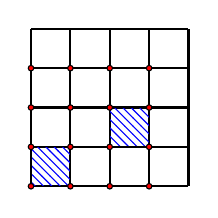
\begin{tikzpicture}[scale = 0.5]
  \draw[step = 1cm, black, thick](0,0) grid (4,4);
\draw[pattern=north west lines, pattern color=blue] (0,0) rectangle (1,1);
\draw[pattern=north west lines, pattern color=blue] (3,1) rectangle (2,2);
\foreach \x in {0,1,2,3}{
  \foreach \y in {0,1,2,3}{
  \draw[fill = red] (\x,\y) circle (2pt);
  } 
}
\end{tikzpicture}
\end{center}
\vspace{-0.25cm}
\caption{Tiling with squares for $m = 4$ and associated cells $C_{4}(0,0)$ and $C_{4}(2,1)$ (blue stripes) and red point of $\mathbb{G}_{m}$.}
\label{figure1}
\end{figure}
\vspace{-1cm}
\paragraph{Discrete setting and binary image}
Using the previous square tiling, we write $S =  \underset{x \in \mathbb{G}_{m}}{\cup}  C_{m}(x)$. We assume to observe $\left(X_{\scriptscriptstyle x}\right)_{x \in \mathbb{G}_{m}}$, which we assume coincides with values of a stationary random field $\left(X_{\scriptscriptstyle x}\right)_{x \in \mathbb{Z}^{2}}$. The stationarity hypothesis means that for all $h \in \mathbb{Z}^{2}$, 
$$\left(X_{x+h}; x \in \mathbb{Z}^{2} \right)\overset{fdd}{=} \left(X_{\scriptscriptstyle x}; x \in \mathbb{Z}^{2} \right),$$ where $fdd$ denotes finite-dimensional distributions. \\
We denote by $\rho(x) :=\text{Cov}\left(X_{\scriptscriptstyle 0}, X_{\scriptscriptstyle x}\right), \; x \in \mathbb{Z}^{2}$, the covariance function of $X$.
\vspace{-1.5cm}
\begin{figure}[H]
    {\includegraphics[scale=0.25]{GaussianUn.pdf}}
    {\includegraphics[scale=0.25]{GaussianZUn.pdf}}
    {\includegraphics[scale=0.25]{GaussianZZZUn.pdf}}
    \vspace{-2cm}
 \caption{Generations of Gaussian random fields with covariance $\rho(x) = e^{-\kappa||x||^{2}}$ with $m = 1024$, and different values for $\kappa$, from left to right $\kappa = 0.01, 0.1, 1$, using the Matlab function \textit{stationary Gaussian process} \cite{MATLAB}.}
\label{fig22}
\end{figure}
Considering a threshold parameter $t \in \mathbb{R}$, we introduce the associated binary \linebreak image $Z^{\scriptscriptstyle (m)}_{t} = \left(\mathbbm{1}_{\left\{X_x \geq t\right\}} \right)_{x \in \mathbb{G}_{m}}$ where each cell $C_{m}(x)$ is associated to black or white according to whether~$X_{x} \geq t$ or $X_{x} \leq t$. 
\subsection{Perimeter of a binary image}\label{methods}
For $t \in \mathbb{R}$, let $Z^{\scriptscriptstyle (m)} = Z^{\scriptscriptstyle (m)}_{t}$ be the  binary image at that given threshold $t \in \mathbb{R}$. Following  the approach  presented in \cite{HermineAgnes},  for each edge $w \in \mathbb{E}_{m}$, we aim to know if  $w$ contributes  to the perimeter of the black component of $Z$. Making use of the additive nature of the perimeter, one can start by computing the oriented perimeter given each direction, horizontal and vertical.
\begin{figure}[H]
\begin{center}
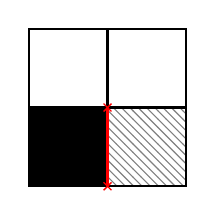
\begin{tikzpicture}
    [
        box/.style={rectangle,draw=black,thick, minimum size=1cm},
    ]
    
    
    here the test 
\foreach \x in {0,1}{
    \foreach \y in {0,1}
        \node[box] at (\x,\y){};
}

\node[box, fill=black] at (0,0){};  
\node[box, pattern = north west lines, pattern color=gray] at (1,0){};  
\draw[step = 1cm, red, thick] (0.5,-0.5) -- (0.5,0.5);
\foreach \x in {0.5}
{
  \draw 
    (\x cm, 0pt) -- (\x cm, 0pt) node[anchor=north] {\scriptsize $\text{\textcolor{red}{}}$};
  \pic[line width=0.5pt,red, rotate = 45] at (\x, 0.5) {mycross};
  \pic[line width=0.5pt,red, rotate = 45] at (\x, -0.5) {mycross};  
}
\end{tikzpicture}
\end{center}
\vspace{-0.25cm}
\caption{The edge $w_{1}(0,0)$ in red belongs to $C_{2}(0,0) \cap C_{2}(1, 0)$, with the cell $C_{2}(0,0)$ colored in black and $C_{2}(1, 0)$ in gray dashed stripes.}
\label{fig1}
\end{figure}
\vspace{-0.5cm}
Following this consideration, one can define the random quantity
\begin{equation}
f_{t}^{\scriptscriptstyle (i)}(x) := \mathbbm{1}_{\left\{\min\left(X_{x}, X_{\scriptscriptstyle x +e_{i}}\right) < t \leq \max\left(X_{x}, X_{\scriptscriptstyle x+e_{i}}\right)\right\}}
\label{fi}
\end{equation}
to compute the contribution of the edge $w_i(x)$ to the perimeter of the black component of~$Z^{\scriptscriptstyle (m)}$. Before stating the definition of the oriented perimeter let us first make an observation that will appear very useful in the rest of the paper.  
\begin{remark}
\label{lemmasommediff}
Let $a,b,t \in \mathbb{R}$, then 
$$\min(a,b) \leq t \leq \max(a,b) \iff\left|2t - (a+b))\right| \leq \left| b-a \right| $$
\end{remark}
\begin{proof}
Let $a,b,t \in \mathbb{R}$,
\begin{figure}[H]
\centering
\begin{tikzpicture}[scale = 1.5]
\draw (-1,0)--(9,0);
\draw (0,-0.08)--(0,0.08);
\draw (8,-0.08)--(8,0.08);
\draw (2.5, -0.08) -- (2.5, 0.08);
\draw (4, -0.08) -- (4, 0.08);
\draw (0,0) node[below]{$\min(a,b)$};
\draw (8,0) node[below]{$\max(a,b)$};
\draw (4,0) node[below]{$\frac{a+b}{2}$};
\draw (2.5,0) node[below]{$t$};
\draw (2.5,-0.6) -- (4,-0.6);
\draw (2.5, -0.6) -- (2.75,-0.5);
\draw (2.5, -0.6) -- (2.75,-0.7);
\draw (4, -0.6) -- (3.75,-0.5);
\draw (4, -0.6) -- (3.75,-0.7);
\draw (0,0.6) -- (8,0.6);
\draw (0, 0.6) -- (0.25,0.5);
\draw (0, 0.6) -- (0.25,0.7);
\draw (8, 0.6) -- (7.75,0.7);
\draw (8, 0.6) -- (7.75,0.5);
\node[text width= 1.6cm, font=\large] at (4,1) {$|b-a|$};
\node[text width= 0.7cm, font=\large] at (3,-1) {$|t -~\frac{a+b}{2}|$};
\end{tikzpicture}
\end{figure}
\vspace{-1cm}
\end{proof}
\begin{Definition}[Oriented perimeter of a binary image $Z^{\scriptscriptstyle (m)}$]\label{defPerimetre}~\\
For $t\in \mathbb{R},$ we denote by $\mathcal{P}_{m}^{\scriptscriptstyle (i)}(t)$ the sum of all contributions over the $i$th direction (vertical for $i = 1$ and horizontal for $i = 2$). Then, the oriented perimeter of the binary image $Z^{\scriptscriptstyle (m)}$ is given by
\begin{equation}
\mathcal{P}_{m}^{\scriptscriptstyle (i)}(t) =~\sum_{\scriptscriptstyle x \in \mathbb{G}^{\scriptscriptstyle (i)}_{m}} f_{t}^{\scriptscriptstyle (i)}(x).
 \label{eq:6}
\end{equation}
Then, the perimeter of $Z^{\scriptscriptstyle (m)}$ is given by $\mathcal{P}_{m}(t) := \mathcal{P}_{m}^{\scriptscriptstyle (1)}(t) + \mathcal{P}_{m}^{\scriptscriptstyle (2)}(t)$.
\end{Definition}
\section{Statistics of the oriented perimeter} 
\subsection{First moment}
Let us start this study by investigating the first moment of the oriented perimeter.
\begin{Proposition}[First moment of the oriented perimeter] 
\label{propFisrtmoment}
We assume that $\left(X_x \right)_{x \in \mathbb{G}_{m}}$ is a stationary Gaussian centered with unit variance random field. Let $i \in \{1,2\}$ and let us denote by  $\rho(e_i) = \text{Cov}\left(X_{\scriptscriptstyle 0}, X_{e_i}\right) \in [-1, 1]$. The expected value of the perimeter in \eqref{eq:6} is  given by $$\mathbb{E}\left(\mathcal{P}_{m}^{\scriptscriptstyle (i)}(t)\right) = m(m-1)\mathbb{E}\left(f^{(i)}(t) \right)$$ where
\begin{itemize}
  \item if $\rho(e_{i}) \in ]-1,1]$, 
    {\small
  \begin{align}
  \label{propEquationFisrtmoment}
  \mathbb{E}\left(f^{(i)}(t) \right) = \mathbb{E}\left(\Phi\left(\dfrac{2t + \sqrt{2(1-\rho(e_i))}|N|}{\sqrt{2(1+\rho(e_i))}}\right)  - \Phi\left(\dfrac{2t - \sqrt{2(1-\rho(e_i))}|N|}{\sqrt{2(1+\rho(e_i))}}\right)\right)
  \end{align}}
with $N \sim \mathcal{N}(0,1)$ and $\Phi$ being the cumulative distribution function of the standard Gaussian. 
\item if $\rho(e_i) = -1, \; \mathbb{E}\left(f^{(i)}(t) \right)= 2\left(1 - \Phi\left(|t|\right)\right).$
  \end{itemize}
\end{Proposition}
\begin{proof}
Let us assume that $\rho(e_{i}) \in ]-1,1]$. Considering the formula for $\mathcal{P}^{\scriptscriptstyle  (i)}_{m}(t)$ and applying the stationarity hypothesis one can write that, 
\begin{equation*}
\mathbb{E}\left(\mathcal{P}^{\scriptscriptstyle  (i)}_{m}(t) \right) = m(m-1)\mathbb{E}\left(f^{(i)}(t)\right),
\label{covarianeproof}
\end{equation*}
 with $\mathbb{E}\left(f^{(i)}(t)\right) = \mathbb{P}\left(\min\left(X_{\scriptscriptstyle 0}, X_{e_i}\right) < t \leq \max\left(X_{\scriptscriptstyle 0}, X_{e_i}\right)\right)$.
We start by applying the following transformation to the Gaussian vector $\left(X_{\scriptscriptstyle 0}, X_{e_i}\right)$,  \begin{equation*} \label{expressions} \Delta^{\scriptscriptstyle (i)}_{\scriptscriptstyle 0} := X_{e_i} - X_{\scriptscriptstyle 0}, \hspace{0.5cm} S^{\scriptscriptstyle (i)}_{\scriptscriptstyle 0} := X_{e_i} + X_{\scriptscriptstyle 0}. \end{equation*} 
The covariance matrix of the new Gaussian vector $\left(\Delta^{\scriptscriptstyle (i)}_{\scriptscriptstyle 0}, S^{\scriptscriptstyle (i)}_{\scriptscriptstyle 0}\right)$ is given by ${\tilde{\Sigma}_{i}(0)~= M\Sigma_{i}(0) M^{\star}}$ with {\small $M = \begin{pmatrix}
-1 & 1 \\
1 & 1  \\
\end{pmatrix}$} and $\Sigma_{i}(0) = \begin{pmatrix} 1 & \rho(e_i) \\
\rho(e_i) & 1  \\ 
\end{pmatrix}.$ Thus, $\tilde{\Sigma}_{i}(0) = \begin{pmatrix}  2(1-\rho(e_i)) & 0 \\ 0 & 2(1+\rho(e_i)  \end{pmatrix}$, which directly  implies that the two variables~$\Delta^{\scriptscriptstyle (i)}_{\scriptscriptstyle 0}$ and $S^{\scriptscriptstyle (i)}_{\scriptscriptstyle 0}$ are independent. Hence, we can write
$\left\{
 \begin{array}{rlc}
  \Delta^{\scriptscriptstyle (i)}_{\scriptscriptstyle 0} & = & \sqrt{2(1-\rho(e_i))}U, \\
  S^{\scriptscriptstyle (i)}_{\scriptscriptstyle 0} & = & \sqrt{2(1+\rho(e_i)}V, 
\end{array}
\right.$ with~$(U, V) \sim \mathcal{N}\left(0, I_{2}\right)$. Thus, applying Remark \ref{lemmasommediff} above we get 
{\small
\begin{align*}
\mathbb{E}\left(f^{(i)}(t)\right) 
& = \mathbb{E}\left(\mathbbm{1}_{\left\{ \left|2t - S^{\scriptscriptstyle (i)}_{\scriptscriptstyle 0}\right| \leq \left|\Delta^{\scriptscriptstyle (i)}_{\scriptscriptstyle 0}\right|\right\}}\right). \\
& = \mathbb{E}\left(\mathbbm{1}_{\left\{\frac{2t - \sqrt{2(1-\rho(e_i))}|U|}{\sqrt{2(1+\rho(e_i))}}  \leq V \leq \frac{2t + \sqrt{2(1-\rho(e_i))}|U|}{\sqrt{2(1+\rho(e_i))}}\right\}}\right), 
\end{align*}}  
thus,
$$\mathbb{E}\left(f^{\scriptscriptstyle (i)}(t)\right) = \mathbb{E}\left(\Phi\left(\dfrac{2t + \sqrt{2(1-\rho(e_i))}|N|}{\sqrt{2(1+\rho(e_i))}}\right)  - \Phi\left(\dfrac{2t - \sqrt{2(1-\rho(e_i))}|N|}{\sqrt{2(1+\rho(e_i))}}\right)\right).$$
Let us now consider the case where $\rho(e_i) = -1$. Then there exists $N \sim \mathcal{N}\left(0,1\right)$ such that $\left(X_{\scriptscriptstyle 0}, X_{e_i}\right) \overset{d}{=} \left(N, -N\right)$. Thus, 
\begin{align*}
\mathbb{E}\left(f^{(i)}(t)\right) & = \mathbb{P}\left(\min\left(N, -N\right) < t \leq \max\left(N, -N\right)\right) \\
& = \mathbb{P}\left(|t| \leq |N|\right) = 2\left(1 - \Phi\left(|t|\right)\right).
\end{align*}
\end{proof}
This result extends the one given in \cite{HermineAgnes} (Proposition 3) since we do not assume here that $\rho(e_i) > 0$. 
\begin{remark}(Degenerate dependence cases.)
\begin{itemize}
\item In the case of a fully dependent field, \textit{i.e}  $\rho(e_i) = 1$, note that $\mathbb{E}\left(\mathcal{P}_{m}^{\scriptscriptstyle (i)}(t) \right) = 0$.
\item In the independent case, \textit{i.e.} $\rho(e_{i}) = \text{Cov}\left(X_{0}, X_{e_i}\right) = 0$, we can write
{\small
\begin{align*}
\mathbb{E}\left(\mathcal{P}^{\scriptscriptstyle  (i)}_{m}(t) \right) & = m(m-1)\mathbb{E}\left(\Phi\left(\sqrt{2}t + |N|\right) - \Phi\left(\sqrt{2}t - |N|\right)\right) = 2m(m-1)\Phi(t)\left(1-\Phi(t)\right), 
\end{align*}}by applying the variable change $ (y, z) \mapsto (\frac{y-z}{\sqrt{2}}, \frac{y+z}{\sqrt{2}})$ to get the second identity. We get the same result as in \cite{Psymetrie} (Proposition \textcolor{blue}{3.1}). \\ As in \cite{Psymetrie} in order to converge towards a non degenerate quantity when $m$ goes to infinity, we have to consider a normalized perimeter thus, dividing the perimeter by the area of the window $S$, considering $\frac{1}{m^2}\mathcal{P}_{m}(t)$.
\end{itemize}
\end{remark}
\paragraph{Total variation.}
\textcolor{red}{
In image processing, the total variation of an image $u \in L^{1}_{loc}(\Omega)$ which is given by $\int_{\Omega}|\nabla u|dx$ is a common and well studied object. It is possible to link this quantity the perimeter of $u$, by applying the coarea formula, $\int_{\Omega}|\nabla u|dx = \int_{\mathbb{R}}\mathcal{P}(t)dt$ with $\mathcal{P}(t)$ being the perimeter associated to the level set of the image $u$ at level $t$. In the following result, by considering Proposition \eqref{propFisrtmoment}, we obtain a simple expression for the first moment of the total variation, and link it directly to the covariance evaluated in the $i$th direction.}
\begin{Proposition}
\label{Variationtotal}
Under the assumptions stated in Proposition \ref{propFisrtmoment}, we get 
\begin{equation}
\label{totalvariation}
\int_{\mathbb{R}} \mathbb{E}\left(\mathcal{P}^{(i)}_{m}(t)\right) dt = \frac{2m(m-1)}{\sqrt{\pi}}\left(\sqrt{1-\rho(e_i)}  \right).
\end{equation}
\end{Proposition}
\begin{proof}
Using the result stated in Proposition \ref{propFisrtmoment}, we get that $\mathbb{E}\left(\mathcal{P}^{\scriptscriptstyle  (i)}_{m}(t) \right)$ is equal to,
{\small
\begin{align*}
\int_{\mathbb{R}} \mathbb{E}\left(\mathcal{P}^{(i)}_{m}(t)\right) dt & = \\
& \hspace{-2cm}\cfrac{m(m-1)}{\sqrt{2\pi}} \int_{\mathbb{R}}\int_{\mathbb{R}} \left(\Phi\left(\dfrac{\sqrt{2}t + \sqrt{1-\rho(e_i)}|u|}{\sqrt{1+\rho(e_i)}}\right) - \Phi\left(\dfrac{\sqrt{2}t - \sqrt{1-\rho(e_i)}|u|}{\sqrt{1+\rho(e_i)}}\right)\right)e^{-\frac{1}{2}u^2}dudt \\
& \hspace{-2cm}=\cfrac{m(m-1)}{2\pi} \int_{\mathbb{R}}\int_{\mathbb{R}}\int_{\mathbb{R}} e^{-\frac{1}{2}u^2}e^{-\frac{1}{2}v^2} \mathbbm{1}_{\left\{\dfrac{\sqrt{2}t - \sqrt{1-\rho(e_i)}|u|}{\sqrt{1+\rho(e_i)}}\leq v \leq\dfrac{\sqrt{2}t + \sqrt{1-\rho(e_i)}|u|}{\sqrt{1+\rho(e_i)}}\right\}} du dv dt ,\\
& \hspace{-2cm}\text{using Fubini-Tonelli Theorem,} \\
& \hspace{-2cm}= \cfrac{m(m-1)}{2\pi}\int_{\mathbb{R}}\int_{\mathbb{R}} e^{-\frac{1}{2}u^2}e^{-\frac{1}{2}v^2} \\
& \hspace{-2cm} \left(\int_{\mathbb{R}} \mathbbm{1}_{\left\{\dfrac{\sqrt{1+\rho(e_i)}v - \sqrt{1-\rho(e_i)}|u|}{\sqrt{2}}\leq t\leq\dfrac{\sqrt{1+\rho(e_i)}v + \sqrt{1-\rho(e_i)}|u|}{\sqrt{2}}\right\}} dt\right) du dv \\
& \hspace{-2cm}= \cfrac{m(m-1)}{2\pi} \int_{\mathbb{R}}\int_{\mathbb{R}} e^{-\frac{1}{2}u^2}e^{-\frac{1}{2}v^2}\left(\dfrac{2|u|\sqrt{1-\rho(e_i)}}{\sqrt{2}}\right)dudv = \frac{2\sqrt{1-\rho(e_i)}}{\sqrt{2}} m(m-1)\underbrace{\mathbb{E}(|U|)}_{\sqrt{\frac{2}{\pi}}}\\
&\hspace{-2cm}=\frac{2}{\sqrt{\pi}}m(m-1)\sqrt{1-\rho(e_i)}.
\end{align*}
}
\end{proof}
\begin{remark}
Using this result, one can define an estimator for $\rho(e_i)$. 
\end{remark}
\textcolor{red}{Let us now study the monotonic properties of the function $\rho \mapsto \mathbb{E}\left(\mathcal{P}^{\scriptscriptstyle (i)}_{m, \rho}(t)\right)$ where $\mathcal{P}^{\scriptscriptstyle (i)}_{m, \rho}$ is the perimeter with respect of the orientation $i$ associated to the Gaussian field of covariance function $\rho$. This result allows us to state that the oriented perimeter is a strictly decreasing function with respect to $\rho$. }
\begin{Proposition}
\label{powertest}
\textcolor{red}{Let $\overline{X}, \tilde{X}$ be two stationary centered Gaussian random fields with unit variance, and $\bar{\rho}, \tilde{\rho}$ their respective covariance structure. For any level $t$, we  have the following result:}
\begin{equation*}
 \text{if} \hspace{0.5cm} \tilde{\rho}(e_i) < \bar{\rho}(e_i) \hspace{0.5cm} \text{then} \hspace{0.5cm}\mathbb{E}\left(\mathcal{P}^{\scriptscriptstyle (i)}_{m, \tilde{\rho}}(t)\right) > \mathbb{E}\left(\mathcal{P}^{\scriptscriptstyle (i)}_{m, \bar{\rho}}(t)\right).
\end{equation*}
\end{Proposition}
\begin{proof}
Let $t \in \mathbb{R}$, We consider the function $h$ defined as follow \begin{align*} 
h: (-1,1) &\longrightarrow \mathbb{R}, \\
x & \longmapsto \mathbb{E}\left(\Phi\left(\dfrac{2t + \sqrt{2(1-x)}|N|}{\sqrt{2(1+x)}}\right) - \Phi\left(\dfrac{2t - \sqrt{2(1-x)}|N|}{\sqrt{2(1+x)}}\right)\right),
\end{align*}
with $N \sim \mathcal{N}\left(0,1\right)$. The derivative of $h$ is equal to 
\begin{align*}
h'(x) & = \mathbb{E}\left( \left(\frac{2t + |N|\sqrt{2(1-x)}}{\sqrt{2(1+x)}}\right)'\Phi'\left(\frac{2t + |N|\sqrt{2(1-x)}}{\sqrt{2(1+x)}}\right)\right. \\
& \hspace{5cm} \left. - \left(\frac{2t - |N|\sqrt{2(1-x)}}{\sqrt{2(1+x)}}\right)'\Phi'\left(\frac{2t - |N|\sqrt{2(1-x)}}{\sqrt{2(1+x)}}\right) \right)\\
& = \mathbb{E}\left(\frac{-2|N| -t\sqrt{2(1-x)}}{2(1+x)\sqrt{1-x^2}}\Phi'\left(\frac{2t + |N|\sqrt{2(1-x)}}{\sqrt{2(1+x)}}\right) \right. \\
& \hspace{6cm}  \left. - \frac{2|N| - t\sqrt{2(1-x)}}{2(1+x)\sqrt{1-x^2}}\Phi'\left(\frac{2t - |N|\sqrt{2(1-x)}}{\sqrt{2(1+x)}}\right) \right) \\
& = \frac{1}{2(1+x)\sqrt{1-x^2}}\mathbb{E}\left(\left(-2|N| -t\sqrt{2(1-x)}\right)\Phi'\left(\frac{2t + |N|\sqrt{2(1-x)}}{\sqrt{2(1+x)}}\right) \right. \\
& \hspace{5.5cm}  \left. - \left(2|N| - t\sqrt{2(1-x)}\right)\Phi'\left(\frac{2t - |N|\sqrt{2(1-x)}}{\sqrt{2(1+x)}}\right) \right) \\
& = \frac{\exp(-t^2/(1+x))}{2\sqrt{2\pi}(1+x)\sqrt{1-x^2}}\\
&\hspace{0.5cm} \mathbb{E}\left(\left(-2|N| -t\sqrt{2(1-x)}\right)\exp\left(\frac{-t|N|\sqrt{2(1-x)}}{1+x}\right)\exp\left(\frac{-N^{2}(1-x)}{2(1+x)}\right)\right. \\
&\hspace{2cm}\left. - \left(2|N| - t\sqrt{2(1-x)}\right)\exp\left(\frac{t|N|\sqrt{2(1-x)}}{1+x}\right)\exp\left(\frac{-N^{2}(1-x)}{2(1+x)}\right)\right) \\
& = \frac{\exp(-t^2/(1+x))}{4\pi(1+x)\sqrt{1-x^2}}\\
&\hspace{0.5cm} \int_{-\infty}^{\infty}\exp\left(-\frac{y^2}{1+x}\right)\left(\left(-2|y| -t\sqrt{2(1-x)}\right)\exp\left(\frac{-t|y|\sqrt{2(1-x)}}{1+x}\right)\right. \\
&\hspace{5cm}\left. - \left(2|y| - t\sqrt{2(1-x)}\right)\exp\left(\frac{t|y|\sqrt{2(1-x)}}{1+x}\right)\right)dy \\ 
& = \frac{\exp(-t^2/(1+x))}{2\pi(1+x)\sqrt{1-x^2}}\exp\left(\frac{t^2(1-x)}{2(1+x)}\right)\\
&\hspace{0.5cm} \int_{0}^{\infty}\left(\left(-2y -t\sqrt{2(1-x)}\right)\exp\left(-\frac{\left(y+t\sqrt{2(1-x)}/2\right)^{2}}{1+x}\right)\right. \\
&\hspace{5cm}\left. - \left(2y - t\sqrt{2(1-x)}\right)\exp\left(-\frac{\left(y-t\sqrt{2(1-x)}/2\right)^{2}}{1+x}\right)\right)dy \\
& = \frac{-\exp(-t^2/(1+x))}{2\pi(1-x)^{1/2}(1+x)^{3/2}}\exp\left(\frac{t^2(1-x)}{2(1+x)}\right)\\
& \hspace{2cm} \left(\int_{\frac{t}{2}\sqrt{2(1-x)}}^{\infty}2z\exp\left(-\frac{z^2}{1+x}\right)dz + \int_{-\frac{t}{2}\sqrt{2(1-x)}}^{\infty}2z\exp\left(-\frac{z^2}{1+x}\right)dz \right)\\
& = \frac{-\exp(-t^2/(1+x))(1+x)}{2\pi(1-x)^{1/2}(1+x)^{3/2}}\\
& = \frac{-\exp(-t^2/(1+x))}{2\pi\sqrt{(1-x^2)}}.
\end{align*}
Since for all $|x| < 1, \; h'(x) < 0$, $h$ is a strictly decreasing function. 
\end{proof}
\begin{remark}
\label{remarkesperancetest}
\textcolor{red}{The function $\rho \mapsto \mathbb{E}\left(\mathcal{P}^{\scriptscriptstyle (i)}_{m, \rho}(t)\right)$ being strictly decreasing, if $\mathbb{E}\left(\mathcal{P}^{\scriptscriptstyle (1)}_{m}(t)\right) \neq \mathbb{E}\left(\mathcal{P}^{\scriptscriptstyle (2)}_{m}(t)\right)$ then~$\rho(e_1) \neq \rho(e_2) $. Now, assume that the field $X$ is isotropic, one consequence would be that $\rho(e_{1}) = \rho(e_{2})$ which implies~$\frac{\mathbb{E}\left(\mathcal{P}^{\scriptscriptstyle (1)}_{m}(t)\right)}{\mathbb{E}\left(\mathcal{P}^{\scriptscriptstyle (2)}_{m}(t)\right)} = 1$. Then, the ratio $\mathcal{P}^{\scriptscriptstyle  (1)}_{m}(t)/\mathcal{P}^{\scriptscriptstyle  (2)}_{m}(t)$ would be distributed around $1$ in the case of isotropy. This consideration will be crucial for the proposed local isotropy testing procedure in the next section.}
\end{remark}
\subsection{Isotropy test using the oriented perimeter}
\label{isotest}
In order to construct a local isotropy test using the oriented perimeter of the field $X$, we first  establish a Central Limit Theorem for the variable $\mathcal{P}^{\scriptscriptstyle (i)}_{m}(t)$. To do that, we have to add some assumptions on $\rho$ the covariance structure of the field $X$.
\begin{enumerate}
  \itemA 
 $\begin{aligned}[t]
 \label{conditionTCL1}
\lim_{m \to \infty} m^{-2}\sum_{x, y \in \mathbb{G}_{m}}\rho(x-y)\; \text{exists}.
\end{aligned}$
\itemA $\begin{aligned}[t]
 \lim_{m \to \infty} m^{-2}\sum_{x, y \in \mathbb{G}_{m}}\rho(x-~y)^{2}\; \text{exists}.
\end{aligned}$
\end{enumerate} 
\textcolor{red}{TCL}
\begin{Theorem}\label{TCL}(Multi-directional multivariate CLT for r-threshold). We consider that $(X_{x})_{x\in \mathbb{G}_{m}}$ is a centered stationary standard Gaussian field. Let $r$ be a positive integer and $t_{1}, \cdots,t_{r} \in \mathbb{R}$. Then, under \textbf{$(A_{1})$} and \textbf{$(A_{2})$},
\begin{equation*}
\frac{1}{m}\left(\begin{pmatrix} \mathcal{P}^{\scriptscriptstyle (1)}_{m}(t_{1}) \\  \vdots \\ \mathcal{P}^{\scriptscriptstyle (1)}_{m}(t_{r}) \\ \mathcal{P}^{\scriptscriptstyle (2)}_{m}(t_{2}) \\  \vdots \\ \mathcal{P}^{\scriptscriptstyle (2)}_{m}(t_{r})  \end{pmatrix} - \begin{pmatrix} \mathbb{E}(\mathcal{P}^{\scriptscriptstyle (1)}_{m}(t_{1}))  \\ \vdots \\ \mathbb{E}(\mathcal{P}^{\scriptscriptstyle (1)}_{m}(t_{r}))\\\mathbb{E}(\mathcal{P}^{\scriptscriptstyle (2)}_{m}(t_{1})) \\ \vdots \\ \mathbb{E}(\mathcal{P}^{\scriptscriptstyle (2)}_{m}(t_{r})) \end{pmatrix}\right) \xrightarrow[m \to \infty]{d} \mathcal{N}\left(0,\,\Sigma_{2r}^{\star}\right),
\end{equation*}
where $\xrightarrow[]{d}$ holds for the convergence in distribution and $\mathcal{N}\left(0,\,\Sigma_{2r}^{\star}\right)$ for the $2r$-dimensional centered Gaussian distribution with covariance matrix $\Sigma^\star_{2r}$ given by
\begin{align}
\label{CovTCL}
\Sigma^{\star}_{2r}(l,i,k,j) & : = \lim_{m \to \infty}\text{Cov}\left(\frac{1}{m}\mathcal{P}^{\scriptscriptstyle (i)}_{m}(t_{l}),  \frac{1}{m}\mathcal{P}^{\scriptscriptstyle (j)}_{m}(t_{k}) \right)
\end{align}
\end{Theorem}
\begin{proof} For the sake of simplicity, we will prove the theorem for $r=1$, the generalized case can be established by following the same procedure. Using the Cramèr-Wold method, we will prove that for each $(a_1, a_2) \in \mathbb{R}^{2}$, we have 
\begin{align*}
\frac{a_{1}}{m}\left(\mathcal{P}^{\scriptscriptstyle (1)}_{m}(t) - \mathbb{E}\left(\mathcal{P}^{\scriptscriptstyle (1)}_{m}(t)\right)\right) + \frac{a_{2}}{m}\left(\mathcal{P}^{\scriptscriptstyle (2)}_{m}(t) - \mathbb{E}\left(\mathcal{P}^{\scriptscriptstyle (2)}_{m}(t)\right)\right) \xrightarrow[m \to \infty]{d} \mathcal{N}\left(0,\,\sigma^{2}(t)\right) 
\end{align*}
with $\sigma^{2}(t) < \infty$. Let~$ t \in \mathbb{R}$, $x=(x_{1}, x_{2}) \in \mathbb{G}_{m}$ and $i \in \{1,2\}$, we recall the notation introduced in \eqref{fi}
\begin{align*}
f_{t}^{\scriptscriptstyle (i)}(x) := \mathbbm{1}_{\left\{\min\left(X_{x+e_{i}}, X_{\scriptscriptstyle x}\right) < t \leq \max\left(X_{x+e_{i}}, X_{\scriptscriptstyle x}\right)\right\}}.
\end{align*}
Let us denote the 4-dimensional Gaussian vector by $\mathbb{X}_{x} = (X_{x_1, x_2}, X_{x_1 + 1, x_2}, X_{x_2, x_1+1}, X_{x_2, x_1} )$ and $g_{t} : \mathbb{R}^{4} \to \mathbb{R}$, 
\begin{align*}
g_{t}\left(u,v, w, z\right) & := a_{1}\mathbbm{1}_{\left\{\min\left(u, v\right) < t \leq \max\left(u, v\right)\right\}} + a_{2}\mathbbm{1}_{\left\{\min\left(w, z\right) < t \leq \max\left(w, z\right)\right\}},
\end{align*}
so that, re-writing the sum we get
\begin{align*} 
\sum_{x \in \mathbb{G}^{(1)}_{m}} g_{t}\left(\mathbb{X}_{x}\right)  & = \sum_{x_1 = 0}^{m-2}\sum_{x_2 = 0}^{m-1} g_{t}\left(\mathbb{X}_{x_{1}, x_{2}}\right)  \\
&=  a_{1}\mathcal{P}^{\scriptscriptstyle (1)}(t) + a_{2}\mathcal{P}^{\scriptscriptstyle (2)}(t).
\end{align*}
Note that $\left|g(t)\right| \leq \left|a_{1}\right| + \left|a_{2}\right|$, thus, $\mathbb{E}\left(g_{t}\left(\mathbb{X}_{\scriptscriptstyle  0, 0}\right)^{2}\right) < (|a_{1}| + |a_{2}|)^{2}$. In order to apply Theorem~$2$ in \cite{arcones} and get the convergence, we should insure that for all $1 \leq p,q \leq 4$, 
\begin{align*}
\lim_{m \to \infty} m^{-2} \sum_{x \in \mathbb{G}^{\scriptscriptstyle (1)}_{m}}\sum_{y \in \mathbb{G}^{\scriptscriptstyle (1)}_{m}} \mathbb{E}\left(\mathbb{X}^{(p)}_{x}\mathbb{X}^{(q)}_{y}\right) \; \text{and} \; \lim_{m \to \infty} m^{-2} \sum_{x \in \mathbb{G}^{\scriptscriptstyle (1)}_{m}}\sum_{y \in \mathbb{G}^{\scriptscriptstyle (1)}_{m}} \left(\mathbb{E}\left(\mathbb{X}^{(p)}_{x}\mathbb{X}^{(q)}_{y}\right)\right)^{2} exist,
\end{align*} 
with $\mathbb{X}^{(i)}_{x}$ being the $i$-coordinate of the $4$-dimensional vector $\mathbb{X}_{x}$. Applying the stationarity hypothesis it amounts to the following, for all $1 \leq i,j \leq 2$,
\begin{align*}
\lim_{m \to \infty} m^{-2}\sum_{x \in \mathbb{G}^{\scriptscriptstyle (i)}_{m}, y \in \mathbb{G}^{\scriptscriptstyle (j)}_{m} }\rho(x-y)  \;  \text{and} \; \lim_{m \to \infty} m^{-2}\sum_{x \in \mathbb{G}^{\scriptscriptstyle (i)}_{m}, y \in \mathbb{G}^{\scriptscriptstyle (j)}_{m} }\rho(x-~y)^{2} exist.
\end{align*} 
Then under $(A1)$ and $(A2)$, we can apply Theorem $2$ in \cite{arcones}, we get that 
\begin{align*}
m^{-1} \sum_{x \in \mathbb{G}^{\scriptscriptstyle (1)}_{m}} g_{\scriptscriptstyle t}\left(\mathbb{X}_{x}\right) - \mathbb{E}\left(g_{\scriptscriptstyle t}\left(\mathbb{X}_{x}\right)\right) \xrightarrow[m \to \infty]{d} \mathcal{N}\left(0,\,\sigma^{2}(t)\right),
\end{align*}
which proves the theorem.
\end{proof}
\textcolor{red}{We are now in position to construct the promised isotropy test.}
\subsection{Perimeter based local isotropy test}
As previously discussed in Remark \ref{remarkesperancetest}, we now aim to build a test using the specific structure of the mean perimeter in the case of local isotropy. Following the idea  in \cite{bierme2019}  we propose a method to test the local isotropy of the field $X$.
Let us consider the null hypothesis
\begin{center}
  $H_{0}$ \, :\; $\rho(e_1) = \rho(e_2)$.
\end{center}
Under $H_{0}$, let us remark that $\mathbb{E}\left(\mathcal{P}^{\scriptscriptstyle  (1) }_{m}(t) \right)= \mathbb{E}\left(\mathcal{P}^{\scriptscriptstyle  (2) }_{m}(t)\right)$ and $\mathbb{V}\left(\mathcal{P}^{\scriptscriptstyle  (1) }_{m}(t) \right)= \mathbb{V}\left(\mathcal{P}^{\scriptscriptstyle  (2) }_{m}(t)\right)$ for all~$t$. Making use of Theorem \ref{TCL}, we have the following normality asymptotic result. 
\begin{Proposition}[Ratio of oriented perimeters]\label{deltamethodgeneralprop} 
Let  $t \in \mathbb{R}$, and $\mathcal{P}^{\scriptscriptstyle  (i) }(t)$ be the oriented perimeter over direction $i$, introduced in Definition \ref{defPerimetre}. Then, it holds that,
\begin{equation*}
\frac{1}{m}\left(\cfrac{\mathcal{P}^{\scriptscriptstyle  (1) }_{m}(t)}{\mathcal{P}^{\scriptscriptstyle  (2)}_{m}(t)} - \cfrac{\mathbb{E}\left(\mathcal{P}^{\scriptscriptstyle  (1) }_{m}(t)\right)}{\mathbb{E}\left(\mathcal{P}^{\scriptscriptstyle  (2)}_{m}(t)\right)} \right)  \xrightarrow[m \to \infty]{d} \mathcal{N}\left(0,  \tilde{\sigma}^{2}(t) \right),
\end{equation*}
with $\tilde{\sigma}^{2}(t) = \frac{(\tilde{\sigma}_{\scriptscriptstyle 1,1}(t)\mu_{2}(t))^{2} - 2\mu_{2}(t)\mu_{1}(t)\tilde{\sigma}_{\scriptscriptstyle 1,2}(t)^{2} +(\tilde{\sigma}_{\scriptscriptstyle 2,2}(t)\mu_{1}(t))^{2}}{\mu_{2}(t)^4}$, $\mu_{i}(t) = \mathbb{E}(f^{(i)}(t))$ as in \eqref{propEquationFisrtmoment} \linebreak and $\tilde{\sigma}_{\scriptscriptstyle 1,1}(t) = \Sigma^{\textcolor{white}{ }^{\star}}_{2}(1,i,1,j)$ as in \eqref{CovTCL}. \\
Furthermore, under $H_{0}$, it holds that
\begin{equation}\label{ratiounderH0}
\frac{1}{m}\left(\cfrac{\mathcal{P}^{\scriptscriptstyle  (1) }_{m}(t)}{\mathcal{P}^{\scriptscriptstyle  (2) }_{m}(t)} - 1 \right)  \xrightarrow[m \to \infty]{d, H_0} \mathcal{N}\left(0,  \tilde{\sigma}_{\scriptscriptstyle H_{0}}^{2}(t)  \right),
\end{equation} 
with $\tilde{\sigma}_{\scriptscriptstyle H_{0}}^{2}(t) = \frac{2\left(\tilde{\sigma}_{\scriptscriptstyle 1,1}^{2}(t) \, - \, \tilde{\sigma}_{\scriptscriptstyle 1,2}^{2}(t)\right)}{\mu_{2}(t)^2}$.
\end{Proposition}
\paragraph{Proposed test with asymptotic level $\alpha$.} Let $t \in \mathbb{R}$,  we denote the ratio by $R_{m}(t) =~\cfrac{\mathcal{P}^{\scriptscriptstyle  (1) }_{m}(t)}{\mathcal{P}^{\scriptscriptstyle  (2) }_{m}(t)}$.
Consider a consistent empirical estimator $\hat{\sigma}^{2}_{m}(t)$ of $\tilde{\sigma}^{2}(t)$. Then, from \ref{deltamethodgeneralprop}, it holds that 
$$ \frac{1}{m\sqrt{\hat{\sigma}^{2}_{m}(t)}}\left(R_{m}(t) - 1 \right)  \xrightarrow[m \to \infty]{d, H_{0}} \mathcal{N}\left(0, 1 \right).$$
Take a confidence level $\alpha \in (0,1)$ and set $q_{1-\frac{\alpha}{2}}$ such that $\mathbb{P}\left(|\mathcal{N}\left(0,1\right)| \leq  q_{1-\frac{\alpha}{2}} \right) = 1 - \frac{\alpha}{2}$. We define the symmetric accessible test $\hat{\phi}_{m}(t)$ with asymptotic level $\alpha$ as 
\begin{equation}
\label{phihat}
\hat{\phi}_{m}(t)= \mathbbm{1}_{\left\{ \frac{1}{m\sqrt{\hat{\sigma}^{2}_{m}(t)}}\left|R_{m}((t) - 1 \right| \geq q_{1- \frac{\alpha}{2}} \right\}}
\end{equation}
Let us now study the consistency of the proposed test statistic, let $H_{1}$ be the alternative hypothesis
\begin{center}
$H_{1}$\, :\; $\rho(e_1) \neq \rho(e_2)$
\end{center} 
\begin{remark}(Consistency of the proposed isotropy test) In Remark \ref{powertest} we showed that the function $\rho \mapsto \mathbb{E}\left(\mathcal{P}^{\scriptscriptstyle (i)}_{m, \rho}(t)\right)$ is strictly decreasing, thus, if $\rho(e_1) \neq \rho(e_2)$ then $\frac{\mathbb{E}\left(\mathcal{P}^{1}_{m}(t)\right)}{\mathbb{E}\left(\mathcal{P}_{m}^{2}(t)\right)} \neq 1$, which implies that $\mathbb{P}_{H_{1}}\left(\hat{\phi}_{m}(t) = 1\right) \to 1$ for $m\to \infty$. 
\end{remark}
\section{Numerical studies}
\subsection{Numerical studies of moments of the estimated perimeter}
Let $X$ be a stationary, isotropic centered Gaussian field with covariance function given by $\rho(x) = (1 -3||x||_{2}/2C + (||x||_{2}/2C)^{3})\mathbbm{1}_{||x||_{2} < C}, x \in \mathbb{R}^2$
Let ${Y(x; a, b, \theta): x \in \mathbb{R}^{2}}$ be a random field equal in distribution to  $\{X(Ax): x\in \mathbb{R}^{2}\}$, where 
\begin{equation}
A:= \begin{pmatrix} a & 0 \\ 0 & b\end{pmatrix} \begin{pmatrix} \cos(\theta) & \sin(\theta) \\ -\sin(\theta) & \cos(\theta)\end{pmatrix} 
\end{equation}
with $a, b \in \mathbb{R}^{2}$ and $\theta \in [0, \pi)$, the field $Y$ is also Gaussian with covariance function given by  $\rho_{X}(x) = (1 - 3||Ax||_{2}/2C + (||Ax||_{2})^{3}/2C^{3})\mathbbm{1}_{||Ax||_{2} < C},$, note that $a\neq b$ if and only if $Y$ is anisotropic. We chose to illustrate the computations of the statistics of the perimeter, using this covariance structure, and the value $\theta = 0$ and $a = 1$. 
\begin{figure}[H]
  \centering
    {\includegraphics[scale=0.3]{EsperanceUnedirection.pdf}}
    \hspace{0.2cm}
 \caption{In each panel, we represent the values of first moment of the oriented perimeter in direction $2$ computed for different values of $b$, the theoretical curve Equation \eqref{propFisrtmoment} is depicted using a blue color (blue) and the empirical values are in orange, the computations were done with a Montecarlo $= 100000$, for different values of $b = 1, 2.5, 5, 10$ and $C = 40$. }
\label{fig2}
\end{figure}

\begin{figure}[H]
  \centering
    {\includegraphics[scale=0.3]{EsperanceUnedirectionfonctionB.pdf}}
    \hspace{0.2cm}
 \caption{In each panel, we represent the values of first moment of the oriented perimeter in direction $2$ computed as a fonction of $b$ for a fixed level $t = 0$, the theoretical curve Equation \eqref{propFisrtmoment} is depicted using a blue color (blue) and the empirical values are in orange, the computations were done with a Montecarlo $= 100000$ and $C = 40$.}
\label{fig2}
\end{figure}


\begin{figure}[H]
  \centering
    {\includegraphics[scale=0.4]{Testanisotropy2.pdf}}
    \hspace{0.2cm} 
 \caption{We represent the values of $\hat{\Phi}_{m}(b)$ see Equation \eqref{phihat} in blue color computed for a Montecarlo $= 2000$, for different values of $b = 1, 1.2, 1.5, 2$ and $C = 40$.}
\label{fig2}
\end{figure}

\begin{figure}[H]
  \centering
    {\includegraphics[scale=0.4]{TestaniRatiopvalue.pdf}}
    \hspace{0.2cm} 
 \caption{$p_{\text{value}} = 2\mathbb{P}\left(N \geq |z|\right)$ with $z = \frac{\mathbb{E}\left(R_{m,n}(t)\right) - 1)}{\sqrt{\hat{\mathbb{V}\left(R_{m, n}(t)\right)}}}$ and $N \sim \mathcal{N}(0,1)$ in blue color computed for a Montecarlo $= 2000$, for different values of $b = 1, 1.1, 1.2, 1.5, 2$ and $C = 40$.}
\label{fig2}
\end{figure}

\begin{center}
\begin{tabular}{|l|c|c|c|c|c|c|c|c|}
\hline
\diagbox{b}{t} & 0.2 &  0.3 &  0.4 &  0.5 &  0.6 &  0.7 &  0.8 &  0.9  \\ \hline
1  & 0.9866 &   0.9638 &  0.9971 &  0.9867 &  0.9674 &  0.9951 &  0.9754 &  0.9918  \\ \hline
1.1 & 0 &  0 &  0 &  0 &  0 &  0 &  0 &  0.0007  \\ \hline
1.2 & 0 &  0 &  0 &  0 &  0 &  0 &  0 &  0   \\ \hline 
1.5 &  0 &  0 &  0 &  0 &  0 &  0 &  0 &  0   \\ \hline
2 &  0 &  0 &  0 &  0 &  0 &  0 &  0 &  0  \\ \hline
\end{tabular}
\end{center}

\begin{figure}[H]
  \centering
    {\includegraphics[scale=0.4]{TestaniRatiopvaluetheta.pdf}}
    \hspace{0.2cm} 
 \caption{We represent $p_{\text{value}} = 2\mathbb{P}\left(N \geq |z|\right)$ with $z = \frac{\mathbb{E}\left(R_{m,n}(t)\right) - 1)}{\sqrt{\hat{\mathbb{V}\left(R_{m, n}(t)\right)}}}$ and $N \sim \mathcal{N}(0,1)$ in blue color computed for a Montecarlo $= 2000$, for different values of $b = 1.1$ and $\theta = \pi/3, \pi/4, \pi/5, \pi/6, \pi/8 $ and $C = 40$.}
\label{fig2}
\end{figure}

\begin{figure}[H]
  \centering
    {\includegraphics[scale=0.4]{TestaniPhi0.pdf}}
    \hspace{0.2cm} 
 \caption{We represent the values of $\hat{\Phi}_{m}$ see Equation \eqref{phihat}, computed as a function of $b$ and a fixed value $t=0$ in blue color for a Montecarlo $= 2000$, and $C = 40$.}
\label{fig2}
\end{figure}

\begin{figure}[H]
  \centering
    {\includegraphics[scale=0.2]{TestaniRatiovsRHO.pdf}}
    {\includegraphics[scale=0.2]{TestaniRatiovsTVA.pdf}}
    \hspace{0.2cm} 
 \caption{We represent the values of the mean of the ratio between the oriented perimeter $\mathbb{E}\left(\frac{\mathcal{P}^{(1)}(0)}{\mathcal{P}^{(2)}(0)}\right)$ in blue and the ratio between of the empirical value for $\hat{\rho(e_i)}$ computed using the first moment of the total variation (\ref{totalvariation}) for different values of $b$, Montecarlo $= 500$, $t = 0$ and $C = 40$.}
\label{fig2}
\end{figure}


\begin{figure}[H]
  \centering
    {\includegraphics[scale=0.3]{imageU.pdf}}
    \hspace{3cm}
    {\includegraphics[scale=0.3]{levelset30000.pdf}}
    \hspace{0.2cm}
 \caption{ Image of level $30000$}
\label{fig2}
\end{figure}

\begin{figure}[H]
  \centering
    {\includegraphics[scale=0.25]{ConfidenceIntervalRDStD.pdf}}
    {\includegraphics[scale=0.25]{BoxplotRDStD.pdf}}
    \hspace{0.2cm}
 \caption{We represent the mean values of the ratio between the two oriented perimeters $\mathcal{P}^{1}, \mathcal{P}^{2}$ for real life data.}
\label{fig2}
\end{figure}


\begin{figure}[H]
  \centering
    {\includegraphics[scale=0.25]{ConfidenceIntervalRDAu.pdf}}
    {\includegraphics[scale=0.25]{BoxplotRDAu.pdf}}
    \hspace{0.2cm}
 \caption{We represent the mean values of the ratio between the two oriented perimeters $\mathcal{P}^{1}, \mathcal{P}^{2}$ for real life data.}
\label{fig2}
\end{figure}
\subsection{Theroretical and numerical study of the covariance of the perimeter}
Let us consider a stationary Gaussian random field $\left(X_{\scriptscriptstyle x}\right)_{x \in \mathbb{Z}^{2}}$ with zero mean and unit variance whose covariance structure is given by $\rho(x) = \text{Cov}\left(X_{\scriptscriptstyle 0}, X_{\scriptscriptstyle x}\right)$ such that $|\rho(e_i)| < 1$.
\begin{Lemma} 
Let $s, t \in \mathbb{R}$, 
\label{CovLemma}
\begin{align*}
\text{Cov}(\mathcal{P}_{m}(t), \mathcal{P}_{m}(s))  & = \sum_{1\leq i,j\leq 2}\text{Cov}(\mathcal{P}_{m}^{\scriptscriptstyle (i)}(t), \mathcal{P}_{m}^{\scriptscriptstyle (j)}(s)) 
\end{align*} 
with 
\begin{align*}
\text{Cov}\left(\mathcal{P}_{m}^{\scriptscriptstyle (i)}(t),\mathcal{P}_{m}^{\scriptscriptstyle (i)}(s) \right) 
& = \sum_{x_{\scriptscriptstyle j}=\left(1-m\right)}^{m-1}\sum_{x_{\scriptscriptstyle i}=\left(2-m\right)}^{m-2}\left(m -|x_{j}|\right)\left(m - 1- |x_{i}|\right) \text{Cov}\left(f_{t}^{\scriptscriptstyle (i)}(0), f_{s}^{\scriptscriptstyle (i)}(x) \right) 
\end{align*} 
for $i,j \in\{1,2\}, i\neq j$, and 
\begin{align*}
\text{Cov}\left(\mathcal{P}_{m}^{\scriptscriptstyle (1)}(t),\mathcal{P}_{m}^{\scriptscriptstyle (2)}(s) \right) 
& = \sum_{x_1=2-m}^{m-1} \sum_{x_2 = 1-m}^{m-2} \left(m-|x_1| - \mathbbm{1}_{x_{1} \leq 0}\right)\left(m-|x_2|-\mathbbm{1}_{x_{2} \geq 0}\right)\text{Cov}\left(f_{t}^{\scriptscriptstyle (1)}(0), f_{s}^{ \scriptscriptstyle (2)}(x) \right).
\end{align*}
\end{Lemma}
\begin{proof}
Let us start with the computation of $\text{Cov}(\mathcal{P}_{m}^{\scriptscriptstyle (1)}(t), \mathcal{P}_{m}^{\scriptscriptstyle (1)}(s))$. 
\begin{align*}
\text{Cov}(\mathcal{P}_{m}^{\scriptscriptstyle (1)}(t), \mathcal{P}_{m}^{\scriptscriptstyle (1)}(s))& = \sum_{x, w_{1}(x) \in \mathbb{E}^{\scriptscriptstyle (1)}_{m}} \sum_{y, w_{1}(y) \in \mathbb{E}^{\scriptscriptstyle (1)}_{m}} \text{Cov}\left(f_{t}^{\scriptscriptstyle (1)}(x), f_{s}^{\scriptscriptstyle (1)}(y) \right).
\end{align*}
By stationarity, one has $\text{Cov}\left(f_{t}^{\scriptscriptstyle (1)}(x), f_{s}^{\scriptscriptstyle (1)}(y) \right)= \text{Cov}\left(f_{t}^{\scriptscriptstyle (1)}(0), f_{s}^{\scriptscriptstyle (1)}(y-x) \right)$, 
\begin{align*}
\text{Cov}\left(\mathcal{P}_{m}^{\scriptscriptstyle (1)}(t),\mathcal{P}_{m}^{\scriptscriptstyle (1)}(s) \right) & = \sum_{x_1 = 0}^{m-2}\sum_{x_2 = 0}^{m-1}\sum_{y_1 = 0}^{m-2}\sum_{y_2 = 0}^{m-1} \text{Cov}\left(f_{t}^{\scriptscriptstyle (1)}(0), f_{s}^{ \scriptscriptstyle (1)}(y-x) \right).
\end{align*}
For $x_1 \in [0,m-2]$ and $z_1 = y_1 - x_1$ one has
\begin{align*} 
\left\{
\begin{array}{rcl}
0 \leq x_1 \leq m-2 \\
0 \leq y_1 \leq m-2 
\end{array}\right.& \Leftrightarrow  \left\{ \begin{array}{rcl}
0 \leq x_1 \leq m-2 \hspace{0.7cm} \\
-x_1 \leq z_1 \leq m-2 - x_1
\end{array}\right. \\
& \Leftrightarrow  \left\{
\begin{array}{rcl}
2-m \leq z_1 \leq m-2 \hspace{2.5cm}  \\
\max(0, -z_1) \leq x_1 \leq \min(m-2 , m-2-z_1)
\end{array}\right..
\end{align*} 
Similarly for $z_2 = y_2 - x_2$ and $x_2 \in [0, m-1]$
\begin{align*}
 \left\{
\begin{array}{rcl}
0 \leq x_2 \leq m-1 \\
0 \leq y_2 \leq m-1 
\end{array}\right. & \Leftrightarrow
\left\{
\begin{array}{rcl}
1-m \leq z_2 \leq m-1 \hspace{2.5cm}  \\
\max(0, -z_2) \leq x_2 \leq \min(m-1 , m-1-z_2).
\end{array}\right., 
\end{align*}
Thus,
\begin{align*}
\text{Cov}\left(\mathcal{P}_{m}^{\scriptscriptstyle (1)}(t),\mathcal{P}_{m}^{\scriptscriptstyle (1)}(s) \right) &  = \sum_{z_{\scriptscriptstyle 1} = \left(2-m\right)}^{m-2}\sum_{z_{\scriptscriptstyle 2}=\left(1-m\right)}^{m-1}\left(m -1 -|z_{1}|\right)\left(m - |z_{2}|\right) \text{Cov}\left(f_{t}^{\scriptscriptstyle (1)}(0), f_{s}^{\scriptscriptstyle (1)}(z) \right). 
\end{align*}
For the last part of \eqref{covariance}, we have still by stationarity
\begin{align*}
\text{Cov}\left(\mathcal{P}_{m}^{\scriptscriptstyle (1)}(t),\mathcal{P}_{m}^{\scriptscriptstyle (2)}(s) \right) & = \sum_{x, w_{1}(x) \subset \text{\larger[1]{$($}}0, m \text{\larger[1]{$)$}}^{2}} \sum_{y, w_{2}(y) \subset \text{\larger[1]{$($}}0, m \text{\larger[1]{$)$}}^{2}} \text{Cov}\left(f_{t}^{\scriptscriptstyle (1)}(0), f_{s}^{ \scriptscriptstyle (2)}(y-x) \right)\\
& =  \sum_{x_1 = 0}^{m-2}\sum_{x_2 = 0}^{m-1}\sum_{y_1 = 0}^{m-1}\sum_{y_2 = 0}^{m-2}\text{Cov}\left(f_{t}^{\scriptscriptstyle (1)}(0), f_{s}^{ \scriptscriptstyle (2)}(y-x) \right)
\end{align*}
Again, considering $z_1 = y_1 - x_1$ and, $z_{2} = y_{2}-x_{2}$, we get
\begin{align*}
\text{Cov}\left(\mathcal{P}_{m}^{\scriptscriptstyle (1)}(t),\mathcal{P}_{m}^{\scriptscriptstyle (2)}(s) \right) & = \sum_{z_1=1}^{m-1}\sum_{z_2 = 0}^{m-2}\left(m-z_1\right)\left(m-z_2-1\right)\text{Cov}\left(f_{t}^{\scriptscriptstyle (1)}(0), f_{s}^{ \scriptscriptstyle (2)}(z) \right)\\
& +  \sum_{z_1=2-m}^{\scriptscriptstyle 0}\sum_{z_2 = 0}^{m-2}\left(m+z_1-1\right)\left(m-z_2-1\right)\text{Cov}\left(f_{t}^{\scriptscriptstyle (1)}(0), f_{s}^{ \scriptscriptstyle (2)}(z) \right)\\
& +  \sum_{z_1=1}^{m-1}\sum_{z_2 = -m+1}^{-1}\left(m-z_1\right)\left(m+z_2\right)\text{Cov}\left(f_{t}^{\scriptscriptstyle (1)}(0), f_{s}^{ \scriptscriptstyle (2)}(z) \right)\\
& + \sum_{z_1=2-m}^{\scriptscriptstyle 0}\sum_{z_2 = -m+1}^{-1} \left(m+z_1-1\right)\left(m+z_2\right)\text{Cov}\left(f_{t}^{\scriptscriptstyle (1)}(0), f_{s}^{ \scriptscriptstyle (2)}(z) \right) \\
& = \sum_{z_1=2-m}^{m-1} \sum_{z_2 = 1-m}^{m-2} \left(m-|z_1| - \mathbbm{1}_{z_{1} \leq 0}\right)\left(m-|z_2|-\mathbbm{1}_{z_{2} \geq 0}\right)\text{Cov}\left(f_{t}^{\scriptscriptstyle (1)}(0), f_{s}^{ \scriptscriptstyle (2)}(z) \right)
\end{align*}
\end{proof}
Getting the value of the covariance $\text{Cov}\left(\mathcal{P}_{m}(t),\mathcal{P}_{m}(s)\right)$ requires the computation of all the \linebreak elements~$\text{Cov}\left(f_{t}^{\scriptscriptstyle (j)}(0), f_{s}^{\scriptscriptstyle (i)}(x)\right)$, $i,j \in\{1,2\}$ which has a two, three or four cells structure, depending on the cardinality of the set $\{C_{m}(0), C_{m}(e_1), C_{m}(x), C_{m}(x+e_i)\}$. 
Figure \ref{configurations} below shows the five types of configurations depending on the orientation $i$ and the position of $x$ on the grid. 
\begin{figure}[H]
\begin{center}
  \begin{subfigure}[b]{0.25\textwidth} 
  \centering
  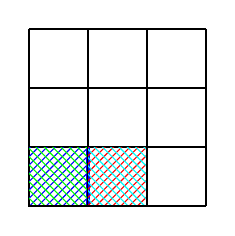
\begin{tikzpicture}[scale = 1.5]
\draw[step = 0.5cm, black, thick](0,0) grid (1.5,1.5);
\draw[step = 2cm, line width =0.5mm, blue] (0.5,0) -- (0.5,0.5);
% \draw[step = 2cm, line width =0.5mm, blue] (1,0) -- (1,0.5);
\draw[pattern=north east lines, pattern color=blue] (0,0) rectangle (0.5,0.5);
\draw[pattern=north west lines, pattern color=green, opacity=1] (0, 0) rectangle (0.5,0.5);
\draw[pattern=north east lines, pattern color=red] (0.5, 0) rectangle (1,0.5);
\draw[pattern=north west lines, pattern color=cyan, opacity=1] (0.5, 0) rectangle (1,0.5);
\end{tikzpicture}
\caption{$i = 1, x = (0,0)$}
\end{subfigure}
\begin{subfigure}[b]{0.25\textwidth} 
  \centering
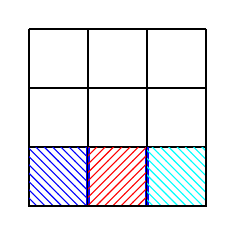
\begin{tikzpicture}[scale = 1.5]
\draw[step = 0.5cm, black, thick](0,0) grid (1.5,1.5);
\draw[step = 2cm, line width =0.5mm, blue] (0.5,0) -- (0.5,0.5);
\draw[step = 2cm, line width =0.5mm, blue] (1,0) -- (1,0.5);
\draw[pattern=north west lines, pattern color=blue] (0,0) rectangle (0.5,0.5);
\draw[pattern=north east lines, pattern color=red] (0.5, 0) rectangle (1,0.5);
\draw[pattern=north west lines, pattern color=cyan, opacity=1] (1, 0) rectangle (1.5,0.5);
\end{tikzpicture}
\caption{$i = 1$, $x = (0,1)$}
\end{subfigure}
\begin{subfigure}[b]{0.25\textwidth} 
  \centering 
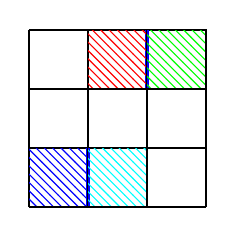
\begin{tikzpicture}[scale = 1.5]
\draw[step = 0.5cm, black, thick](0,0) grid (1.5,1.5);
\draw[step = 2cm, line width =0.5mm, blue] (0.5,0) -- (0.5,0.5);
\draw[step = 2cm, line width =0.5mm, blue] (1,1) -- (1,1.5);
\draw[pattern=north west lines, pattern color=blue] (0,0) rectangle (0.5,0.5);
\draw[pattern=north west lines, pattern color=cyan, opacity=1] (0.5, 0) rectangle (1,0.5);
\draw[pattern=north west lines, pattern color=green, opacity=1] (1.5, 1.5) rectangle (1,1);
\draw[pattern=north west lines, pattern color=red, opacity=1] (0.5, 1)  rectangle (1, 1.5);
\end{tikzpicture}
\caption{$i = 1, x = (1,2)$}
\end{subfigure}
  \hspace{0.5cm}
\begin{subfigure}[b]{0.25\textwidth} 
\centering
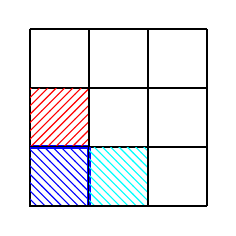
\begin{tikzpicture}[scale =1.5]
\draw[step = 0.5cm, black, thick](0,0) grid (1.5,1.5);
\draw[step = 2cm, line width =0.5mm, blue] (0.5,0) -- (0.5,0.5);
\draw[step = 2cm, line width =0.5mm, blue] (0,0.5) -- (0.5,0.5);
\draw[pattern=north west lines, pattern color=blue] (0,0) rectangle (0.5,0.5);
\draw[pattern=north east lines, pattern color=red] (0, 0.5) rectangle (0.5,1);
\draw[pattern=north west lines, pattern color=cyan, opacity=1] (0.5, 0) rectangle (1,0.5);
\end{tikzpicture}
\caption{$i = 2, x = (0,0)$}
\end{subfigure}
\begin{subfigure}[b]{0.25\textwidth} 
\centering 
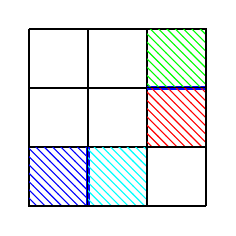
\begin{tikzpicture}[scale = 1.5]
\draw[step = 0.5cm, black, thick](0,0) grid (1.5,1.5);
\draw[step = 2cm, line width =0.5mm, blue] (0.5,0) -- (0.5,0.5);
\draw[step = 2cm, line width =0.5mm, blue] (1,1) -- (1.5,1);
\draw[pattern=north west lines, pattern color=blue] (0,0) rectangle (0.5,0.5);
\draw[pattern=north west lines, pattern color=cyan, opacity=1] (0.5, 0) rectangle (1,0.5);
\draw[pattern=north west lines, pattern color=green, opacity=1] (1.5, 1.5) rectangle (1,1);
\draw[pattern=north west lines, pattern color=red, opacity=1] (1, 0.5)  rectangle (1.5, 1);
\end{tikzpicture}
\caption{$i = 2, z = (2,1)$}
\end{subfigure}
\end{center}
\caption{Illustration of the two, three and four cells configuration involved in the computation of $\text{Cov}\left(f_{t}^{\scriptscriptstyle (1)}(0), f_{s}^{ \scriptscriptstyle (i)}(x)\right)$ in Lemma \ref{CovLemma}.}
\label{configurations}
\end{figure}
Let us first start with the two cells case, which appears in the computation of the term $\text{Cov}\left(f_{t}^{\scriptscriptstyle (1)}(0), f_{s}^{\scriptscriptstyle (1)}(0)\right)$. Applying the same strategy we used to compute the first moment in Proposition \ref{propFisrtmoment}, we get the next result. \\
\begin{Lemma}(Computation of the two cells contribution)
\begin{align*}
\text{Cov}\left(f_{t}^{\scriptscriptstyle (1)}(0), f_{s}^{\scriptscriptstyle (1)}(0)\right) & = \mathbb{E}\left(\mathbbm{1}_{\left\{\min(X_{\scriptscriptstyle 0}, X_{\scriptscriptstyle  e_1}) \leq t \leq \max(X_{\scriptscriptstyle 0}, X_{e_1})\right\}}\mathbbm{1}_{\left\{\min(X_{\scriptscriptstyle 0}, X_{ \scriptscriptstyle  e_1}) \leq s \leq \max(X_{\scriptscriptstyle 0}, X_{\scriptscriptstyle e_1}) \right\}}\right) \\
& - \mathbb{E}\left(\mathbbm{1}_{\left\{\min(X_{\scriptscriptstyle 0}, X_{e_1}) \leq t \leq \max(X_{\scriptscriptstyle 0}, X_{e_1})\right\}}\right)\mathbb{E}\left(\mathbbm{1}_{\left\{\min(X_{\scriptscriptstyle 0}, X_{e_1}) \leq s \leq \max(X_{\scriptscriptstyle 0}, X_{e_1})\right\}}\right),
\end{align*}
where, 
{\small
\begin{align*}
\mathbb{E}\left(\mathbbm{1}_{\left\{\min(X_{\scriptscriptstyle 0}, X_{\scriptscriptstyle  e_1}) \leq t \leq \max(X_{\scriptscriptstyle 0}, X_{e_1})\right\}}\mathbbm{1}_{\left\{\min(X_{\scriptscriptstyle 0}, X_{ \scriptscriptstyle  e_1}) \leq s \leq \max(X_{\scriptscriptstyle 0}, X_{\scriptscriptstyle e_1}) \right\}}\right) & = \\
& \hspace{-9cm}\mathbb{E}\left(\left(\Phi\left(\dfrac{\sqrt{2}\max\left(t,s\right) + \sqrt{1-\rho(e_1)}|Z|}{\sqrt{1+\rho(e_1)}}\right)  - \Phi\left(\dfrac{\sqrt{2}\min\left(t,s\right) - \sqrt{1-\rho(e_1)}|Z|}{\sqrt{1+\rho(e_1)}}\right)\right)\right. \\
& \hspace{-1cm} \left.\mathbbm{1}_{\left\{(|s-t| \leq |Z|\sqrt{2(1-\rho(e_1))}\right\}}\right)
\end{align*}}
with $Z \sim \mathcal{N}(0,1)$. 
\end{Lemma}
Let $x \in \mathbb{Z}^{2}$ such that the covariance matrix $\Sigma_{i}(x)$ of the Gaussian vector $\left(X_{\scriptscriptstyle 0}, X_{e_1}, X_{\scriptscriptstyle x}, X_{x+e_i}\right)$ is invertible, 
$$\Sigma_{i}(x) = \begin{pmatrix} 1 & \rho(e_1) & \rho(x) & \rho(x+e_i)\\
\rho(e_1) & 1 & \rho(x-e_1) &  \rho(x+e_i- e_1) \\ 
\rho(x) & \rho(x-e_1) & 1 & \rho(e_i) \\
\rho(x+e_i) & \rho(x+e_i-e_1) & \rho(e_i) & 1 \end{pmatrix}.$$
Let us define the following quantities   \begin{equation} \label{expressions} \Delta^{\scriptscriptstyle (i)}_{\scriptscriptstyle x} := X_{x+e_i} - X_{\scriptscriptstyle x}, \hspace{0.5cm} S^{\scriptscriptstyle (i)}_{\scriptscriptstyle x} := X_{x+e_i} + X_{\scriptscriptstyle x},\end{equation}
\begin{center}
$\Delta \rho(x) = \rho(x-e_1)-\rho(x)$ and $S\rho(x)  =  \rho(x-e_1)+\rho(x)$.
\end{center}
\begin{Proposition}\label{PropositionFourCell}(Computation of the four cell contribution).
Let $x \in \mathbb{Z}^{2}$ such that the covariance matrix $\Sigma_{i}(x)$ of the Gaussian vector $\left(X_{\scriptscriptstyle 0}, X_{e_1}, X_{\scriptscriptstyle x}, X_{x+e_i}\right)$ is invertible, we introduce the following quantities that are non zeros, \\ 
$\left\{
 \begin{array}{rlc}
 \sigma^{\scriptscriptstyle (-)}_{1} & = &  \sqrt{2(1-\rho(e_1))} \\
 \sigma^{\scriptscriptstyle (+)}_{1} & = & \sqrt{2(1+\rho(e_1))} \\
 \end{array}\right.$ \\
 $\left\{
 \begin{array}{rlc}
   \pi^{\scriptscriptstyle(-, i)}_{U}(x) & = & \hspace{-3cm} \frac{1}{\sigma^{\scriptscriptstyle (-)}_{1}}\left(\Delta \rho(x+e_i) -\Delta \rho(x)\right)  \\
   \pi^{\scriptscriptstyle(-, i)}_{V}(x) & = & \hspace{-3cm} \frac{1}{\sigma^{\scriptscriptstyle (+)}_{1}}\left(S\rho(x+e_i)-S\rho(x)\right)  \\
   \pi^{\scriptscriptstyle(-, i)}_{W}(x)& = & \left(2(1 - \rho(e_{i})) - \pi^{\scriptscriptstyle(-, i)}_{U}(x)^{2} - \pi^{\scriptscriptstyle(-, i)}_{V}(x)^{2}\right)^{\scriptscriptstyle (1/2)}, \end{array}\right.$ \\
    $\left\{
 \begin{array}{rlc}
   \pi^{\scriptscriptstyle(+, i)}_{U}(x) & = & \hspace{-5cm} \frac{1}{\sigma^{\scriptscriptstyle (-)}_{1}}\left(\Delta \rho(x) + \Delta \rho(x+e_i)\right) \\
    \pi^{\scriptscriptstyle(+, i)}_{V}(x) & = & \hspace{-5cm} \frac{1}{\sigma^{\scriptscriptstyle (+)}_{1}}\left(S \rho(x) + S\rho(x+e_i)\right) \\
     \pi^{\scriptscriptstyle(+, i)}_{W}(x) & = & \hspace{-1.5cm} \frac{-1}{\pi^{\scriptscriptstyle(-, i)}_{W}(x)}\left(\pi^{\scriptscriptstyle(-, i)}_{U}(x)\pi^{\scriptscriptstyle(+, i)}_{U}(x) + \pi^{\scriptscriptstyle(-, i)}_{V}(x)\pi^{\scriptscriptstyle(+, i)}_{V}(x)\right) \\
   \pi^{\scriptscriptstyle(+, i)}_{Z}(x)& = & \left(2(1 + \rho(e_i)) - \pi^{\scriptscriptstyle(+, i)}_{U}(x)^{2} - \pi^{\scriptscriptstyle(+, i)}_{V}(x)^{2} - \pi^{\scriptscriptstyle(+, i)}_{W}(x)^{2}\right)^{\scriptscriptstyle (1/2)}.
\end{array}\right.$ \\
then,
{\small
 \begin{align}
\label{covconf}
\text{Cov}\left(f_{t}^{\scriptscriptstyle (1)}(0), f_{s}^{ \scriptscriptstyle (i)}(x)\right) & = 
\mathbb{E}\left(\mathbbm{1}_{\left\{ |2t - \sigma^{\scriptscriptstyle (+)}_{1}V| \leq |\sigma^{\scriptscriptstyle (-)}_{1}U|\right\}}\right. \nonumber\\
& \hspace{1cm} \left. \left|\Phi_{ \pi^{\scriptscriptstyle(+, i)}_{Z}(x)}\left( 2s - \frac{2\Delta \rho(x) }{\sigma^{\scriptscriptstyle (-)}_{1}} U - \frac{2S\rho(x)}{\sigma^{\scriptscriptstyle (+)}_{1}}V - \left( \pi^{\scriptscriptstyle(+, i)}_{W}(x) -  \pi^{\scriptscriptstyle(-, i)}_{W}(x)\right) W \right) \right. \right.  \nonumber \\
& \hspace{1cm} \left. \left.  - \Phi_{ \pi^{\scriptscriptstyle(+, i)}_{Z}(x)}\left( 2s - \frac{2\Delta \rho(x+e_i) }{\sigma^{\scriptscriptstyle (-)}_{1}}U - \frac{2S \rho(x+e_i) }{\sigma^{\scriptscriptstyle (+)}_{1}}V - \left( \pi^{\scriptscriptstyle(+, i)}_{W}(x) +  \pi^{\scriptscriptstyle(-, i)}_{W}(x) \right)W \right)  \right| \right) \nonumber \\
& \hspace{4cm}  - \mathbb{E}\left(f_{t}^{\scriptscriptstyle (1)}(0)\right)\mathbb{E}\left(f_{s}^{ \scriptscriptstyle (i)}(x)\right).
\end{align}}
% {\small 
% \begin{align}
% \label{Thisthofour}
% \mathbb{E}\left(\mathbbm{1}_{\left\{ \left|2t - S^{\scriptscriptstyle (1)}_{\scriptscriptstyle 0}\right| \leq \left|\Delta^{\scriptscriptstyle (1)}_{\scriptscriptstyle 0}\right|\right\}}\mathbbm{1}_{\left\{ \left|2s - S^{\scriptscriptstyle i}_{\scriptscriptstyle x}\right| \leq \left|\Delta^{\scriptscriptstyle (i)}_x\right| \right\}}\right) & = \mathbb{E}\left(\mathbbm{1}_{\left\{ |2t - \sigma^{\scriptscriptstyle (+)}_{1}V| \leq |\sigma^{\scriptscriptstyle (-)}_{1}U|\right\}}\right. \nonumber\\
% & \hspace{-6cm} \left. \left|\Phi_{ \pi^{\scriptscriptstyle(+, i)}_{Z}(x)}\left( 2s - \frac{2\Delta \rho(x) }{\sigma^{\scriptscriptstyle (-)}_{1}} U - \frac{2S\rho(x)}{\sigma^{\scriptscriptstyle (+)}_{1}}V - \left( \pi^{\scriptscriptstyle(+, i)}_{W}(x) -  \pi^{\scriptscriptstyle(-, i)}_{W}(x)\right) W \right) \right. \right.  \nonumber \\
% & \hspace{-4cm}\left. \left.  - \Phi_{ \pi^{\scriptscriptstyle(+, i)}_{Z}(x)}\left( 2s - \frac{2\Delta \rho(x+e_i) }{\sigma^{\scriptscriptstyle (-)}_{1}}U - \frac{2S \rho(x+e_i) }{\sigma^{\scriptscriptstyle (+)}_{1}}V - \left( \pi^{\scriptscriptstyle(+, i)}_{W}(x) +  \pi^{\scriptscriptstyle(-, i)}_{W}(x) \right)W \right)  \right| \right)
% \end{align}
% }
with $\Phi_{\pi^{\scriptscriptstyle(+, i)}_{Z}(x)}$ the cumulative distribution function of $Z \sim \mathcal{N}(0, (\pi^{\scriptscriptstyle(+, i)}_{Z}(x))^{2})$, 
\end{Proposition}
\begin{proof}(Proof of Proposition \ref{PropositionFourCell})
Let us consider the Gaussian vector $\left(X_{\scriptscriptstyle 0}, X_{e_1}, X_{\scriptscriptstyle x}, X_{x+e_i}\right)$ of covariance matrix given by $$\Sigma_{i}(x) = \begin{pmatrix} 1 & \rho(e_1) & \rho(x) & \rho(x+e_i)\\
\rho(e_1) & 1 & \rho(x-e_1) &  \rho(x+e_i- e_1) \\ 
\rho(x) & \rho(x-e_1) & 1 & \rho(e_i) \\
\rho(x+e_i) & \rho(x+e_i-e_1) & \rho(e_i) & 1 \end{pmatrix}.$$ 
Let us define the following quantities   \begin{equation} \label{expressions} \Delta^{\scriptscriptstyle (i)}_{\scriptscriptstyle x} := X_{x+e_i} - X_{\scriptscriptstyle x}, \hspace{0.5cm} S^{\scriptscriptstyle (i)}_{\scriptscriptstyle x} := X_{x+e_i} + X_{\scriptscriptstyle x},\end{equation}
\begin{center}
$\Delta \rho(x) = \rho(x-e_1)-\rho(x)$ and $S\rho(x)  =  \rho(x-e_1)+\rho(x)$.
\end{center}
The covariance matrix of the Gaussian vector $\left(\Delta^{\scriptscriptstyle (1)}_{\scriptscriptstyle 0}, S^{\scriptscriptstyle (1)}_{\scriptscriptstyle 0}, \Delta^{\scriptscriptstyle (i)}_{\scriptscriptstyle x}, S^{\scriptscriptstyle (i)}_{\scriptscriptstyle x}\right)$ is equal to ${\tilde{\Sigma}_{i}(x)~= M\Sigma_{i}(x) M^{\star}}$ with {\small $M = \begin{pmatrix}
-1 & 1 & 0 &  0 \\
1 & 1 & 0 &  0 \\
0& 0 & -1 &  1 \\
0 & 0 & 1 & 1
\end{pmatrix}$}. Then $\tilde{\Sigma}_{i}(x) = \begin{pmatrix} A_{1} & B_{i}(x) \\ B^{\star}_{i}(x) & A_{i} \end{pmatrix}$
with 
$A_{i} = \begin{pmatrix} 2(1-\rho(e_i)) & 0 \\ 0 & 2(1+\rho(e_i))\end{pmatrix}$ and \linebreak {\small $B_{i}(x) =~\begin{pmatrix} \Delta \rho(x+e_i) - \Delta \rho(x)&    \Delta \rho(x) + \Delta \rho(x+e_i) \\ 
 S\rho(x+e_i)- S\rho(x) &  S\rho(x) + S\rho(x+e_i) 
 \end{pmatrix}$}. The quantity we aim to compute is 
{\small
\begin{align}
\label{covconf}
\text{Cov}\left(f_{t}^{\scriptscriptstyle (1)}(0), f_{s}^{ \scriptscriptstyle (i)}(x)\right) & = \nonumber \\
& \hspace{-2.7cm} \mathbb{E}\left(\mathbbm{1}_{\left\{\min(X_{\scriptscriptstyle 0}, X_{e_1}) \leq t \leq \max(X_{\scriptscriptstyle 0}, X_{e_1})\right\}}\mathbbm{1}_{\left\{\min(X_{\scriptscriptstyle x}, X_{x+e_i}) \leq s \leq \max(X_{\scriptscriptstyle x}, X_{x+e_i}) \right\}}\right) \nonumber\\
& \hspace{1cm} - \mathbb{E}\left(\mathbbm{1}_{\left\{\min(X_{\scriptscriptstyle 0}, X_{e_1}) \leq t \leq \max(X_{\scriptscriptstyle 0}, X_{e_1})\right\}}\right)\mathbb{E}\left(\mathbbm{1}_{\left\{\min(X_{\scriptscriptstyle 0}, X_{e_i}) \leq s \leq \max(X_{\scriptscriptstyle 0}, X_{e_i})\right\}}\right).
\end{align}}Considering the first part of the previous equation, and applying Lemma \ref{lemmasommediff}
{\small
\begin{align*}
\mathbb{E}\left(\mathbbm{1}_{\left\{\min(X_{\scriptscriptstyle 0}, X_{e_1}) \leq t \leq \max(X_{\scriptscriptstyle 0}, X_{e_1})\right\}}\mathbbm{1}_{\left\{\min(X_{\scriptscriptstyle x}, X_{x+e_i}) \leq s \leq \max(X_{\scriptscriptstyle x}, X_{x+e_i}) \right\}}\right)\\
& \hspace{-3cm}= \mathbb{E}\left(\mathbbm{1}_{\left\{ \left|2t - S^{\scriptscriptstyle (1)}_{\scriptscriptstyle 0}\right| \leq \left|\Delta^{\scriptscriptstyle (1)}_{\scriptscriptstyle 0}\right|\right\}}\mathbbm{1}_{\left\{ \left|2s - S^{\scriptscriptstyle (i)}_{\scriptscriptstyle x}\right| \leq \left|\Delta^{\scriptscriptstyle (i)}_x\right| \right\}}\right).
\end{align*}} We know that $|\rho(e_1)| < 1$, and that $\tilde{\Sigma}_{i}(x)$ is invertible, thus, the Cholesky decomposition of $\tilde{\Sigma}_{i}(x)$ allows us to get the expression of the Gaussian vector $\left(\Delta^{\scriptscriptstyle (1)}_{\scriptscriptstyle 0},S^{\scriptscriptstyle (1)}_{\scriptscriptstyle 0},\Delta^{\scriptscriptstyle (i)}_{\scriptscriptstyle x},S^{\scriptscriptstyle (i)}_{\scriptscriptstyle x} \right)$ in a new basis $\left(U,V,W,Z\right)$ with $\left(U, V, W, Z\right) \sim \mathcal{N}\left(0,I_{4}\right)$. We get the following decomposition \\ 
$\left\{
  \begin{array}{rlc}
  \Delta^{\scriptscriptstyle (1)}_{\scriptscriptstyle 0} & = & \sigma^{\scriptscriptstyle (-)}_{1}U,  \textcolor{white}{+  \pi^{\scriptscriptstyle(+, i)}_{V}(x) V  } \\
  S^{\scriptscriptstyle (1)}_{\scriptscriptstyle 0} & = & \textcolor{white}{\sigma^{\scriptscriptstyle (-)}_{1}U,} \sigma^{\scriptscriptstyle (+)}_{1}V,
  \end{array}\right.$
  \hspace{-0.9cm}\\
  $\left\{
  \begin{array}{rlc}
  \Delta^{\scriptscriptstyle (i)}_{\scriptscriptstyle  x}& = &  \pi^{\scriptscriptstyle(-, i)}_{U}(x)U +  \pi^{\scriptscriptstyle(-, i)}_{V}(x) V +  \pi^{\scriptscriptstyle(-, i)}_{W}(x) W, \textcolor{white}{ + \pi^{\scriptscriptstyle(+, i)}_{Z}(x)Z, } \\
  S^{\scriptscriptstyle (i)}_{\scriptscriptstyle x} & = &    \pi^{\scriptscriptstyle(+, i)}_{U}(x)U +  \pi^{\scriptscriptstyle(+, i)}_{V}(x) V +  \pi^{\scriptscriptstyle(+, i)}_{W}(x) W +  \pi^{\scriptscriptstyle(+, i)}_{Z}(x)Z, \text{with}
\end{array}\right.$ \\
$\left\{
 \begin{array}{rlc}
 \sigma^{\scriptscriptstyle (-)}_{1} & = &  \sqrt{2(1-\rho(e_1))} \\
 \sigma^{\scriptscriptstyle (+)}_{1} & = & \sqrt{2(1+\rho(e_1))} \\
 \end{array}\right.$ \\
 $\left\{
 \begin{array}{rlc}
   \pi^{\scriptscriptstyle(-, i)}_{U}(x) & = & \frac{1}{\sigma^{\scriptscriptstyle (-)}_{1}}\left(\Delta \rho(x+e_i) -\Delta \rho(x)\right) \\
   \pi^{\scriptscriptstyle(-, i)}_{V}(x) & = &  \frac{1}{\sigma^{\scriptscriptstyle (+)}_{1}}\left(S\rho(x+e_i)-S\rho(x)\right)  \\
   \pi^{\scriptscriptstyle(-, i)}_{W}(x)& = & \left(2(1 - \rho(e_{i})) - \pi^{\scriptscriptstyle(-, i)}_{U}(x)^{2} - \pi^{\scriptscriptstyle(-, i)}_{V}(x)^{2}\right)^{\scriptscriptstyle (1/2)} \end{array}\right.$ \\
    $\left\{
 \begin{array}{rlc}
   \pi^{\scriptscriptstyle(+, i)}_{U}(x) & = &  \frac{1}{\sigma^{\scriptscriptstyle (-)}_{1}}\left(\Delta \rho(x) + \Delta \rho(x+e_i)\right) \\
    \pi^{\scriptscriptstyle(+, i)}_{V}(x) & = & \frac{1}{\sigma^{\scriptscriptstyle (+)}_{1}}\left(S \rho(x) + S\rho(x+e_i)\right) \\
     \pi^{\scriptscriptstyle(+, i)}_{W}(x) & = & \frac{-1}{\pi^{\scriptscriptstyle(-, i)}_{W}(x)}\left(\pi^{\scriptscriptstyle(-, i)}_{U}(x)\pi^{\scriptscriptstyle(+, i)}_{U}(x) + \pi^{\scriptscriptstyle(-, i)}_{V}(x)\pi^{\scriptscriptstyle(+, i)}_{V}(x)\right) \\
   \pi^{\scriptscriptstyle(+, i)}_{Z}(x)& = & \left(2(1 + \rho(e_i)) - \pi^{\scriptscriptstyle(+, i)}_{U}(x)^{2} - \pi^{\scriptscriptstyle(+, i)}_{V}(x)^{2} - \pi^{\scriptscriptstyle(+, i)}_{W}(x)^{2}\right)^{\scriptscriptstyle (1/2)}.
\end{array}\right.$ \\
Developing the indicator function, we get the following expression
{\small
\begin{align*}
\mathbbm{1}_{\left\{ |2s - S^{i}_{\scriptscriptstyle x}| \leq |\Delta^{\scriptscriptstyle(i)}_ {\scriptscriptstyle x}| \right\}}
& = \mathbbm{1}_{\big\{ 2s -  \pi^{\scriptscriptstyle(+, i)}_{U}(x)U -  \pi^{\scriptscriptstyle(+, i)}_{V}(x) V -  \pi^{\scriptscriptstyle(+, i)}_{W}(x) W  - |\Delta^{\scriptscriptstyle(i)}_ {\scriptscriptstyle x}| \leq \pi^{\scriptscriptstyle(+, i)}_{Z}(x)Z} \\ 
& \hspace{3cm} _{\leq 2s -  \pi^{\scriptscriptstyle(+, i)}_{U}(x)U -  \pi^{\scriptscriptstyle(+, i)}_{V}(x) V -  \pi^{\scriptscriptstyle(+, i)}_{W}(x) W + |\Delta^{\scriptscriptstyle(i)}_ {\scriptscriptstyle x}| \big\}}
\end{align*}}Thus, 
\begin{align*}
\mathbb{E}\left(\mathbbm{1}_{\left\{ |2t - S^{\scriptscriptstyle (1)}_{\scriptscriptstyle 0}| \leq |\Delta^{\scriptscriptstyle (1)}_{\scriptscriptstyle 0}|\right\}}\mathbbm{1}_{\left\{ |2s - S^{\scriptscriptstyle (i)}_{\scriptscriptstyle x}| \leq |\Delta^{\scriptscriptstyle (i)}_ {\scriptscriptstyle x}| \right\}}\right)\\
&\hspace{-6.5cm} = \mathbb{E}\left(\mathbbm{1}_{\left\{ |2t - S^{\scriptscriptstyle (1)}_{\scriptscriptstyle 0}| \leq |\Delta^{\scriptscriptstyle (1)}_{\scriptscriptstyle 0}|\right\}}\mathbbm{1}_{\big\{ 2s -  \pi^{\scriptscriptstyle(+, i)}_{U}(x)U -  \pi^{\scriptscriptstyle(+, i)}_{V}(x) V -  \pi^{\scriptscriptstyle(+, i)}_{W}(x) W  - |\Delta^{\scriptscriptstyle(i)}_ {\scriptscriptstyle x}| \leq \pi^{\scriptscriptstyle(+, i)}_{Z}(x)Z} \right.  \\  
& \hspace{3cm}\left. _{\leq 2s -  \pi^{\scriptscriptstyle(+, i)}_{U}(x)U -  \pi^{\scriptscriptstyle(+, i)}_{V}(x) V -  \pi^{\scriptscriptstyle(+, i)}_{W}(x) W + |\Delta^{\scriptscriptstyle(i)}_ {\scriptscriptstyle x}| \big\}}\right)\\
& \hspace{-6.5cm} \text{The variable}\; \pi^{\scriptscriptstyle(+, i)}_{Z}Z \; \text{follows a} \; \mathcal{N}\left(0, \pi^{\scriptscriptstyle(+, i)}_{Z}(x)^{2}\right) \text{and} \; \text{$\Phi_{\pi^{\scriptscriptstyle(+, i)}_{Z}(x)}$ being an increasing function, we get}\\
& \hspace{-6.5cm} = \mathbb{E}\left(\mathbbm{1}_{\left\{ |2t - \sigma^{\scriptscriptstyle (+)}_{1}V| \leq |\sigma^{\scriptscriptstyle (-)}_{1}U|\right\}}\right. \\
&\hspace{-4cm} \left. \left|\Phi_{ \pi^{\scriptscriptstyle(+, i)}_{Z}(x)}\left( 2s -  \pi^{\scriptscriptstyle(+, i)}_{U}(x)U -  \pi^{\scriptscriptstyle(+, i)}_{V}(x) V -  \pi^{\scriptscriptstyle(+, i)}_{W}(x) W  + \Delta^{\scriptscriptstyle(i)}_ {\scriptscriptstyle x}  \right) \right. \right.  \nonumber \\
& \hspace{-4cm}\left. \left.  - \Phi_{ \pi^{\scriptscriptstyle(+, i)}_{Z}(x)}\left( 2s -  \pi^{\scriptscriptstyle(+, i)}_{U}(x)U -  \pi^{\scriptscriptstyle(+, i)}_{V}(x) V -  \pi^{\scriptscriptstyle(+, i)}_{W}(x) W  - \Delta^{\scriptscriptstyle(i)}_ {\scriptscriptstyle x} \right)  \right| \right) \\
& \hspace{-6.5cm} = \mathbb{E}\left(\mathbbm{1}_{\left\{ |2t - \sigma^{\scriptscriptstyle (+)}_{1}V| \leq |\sigma^{\scriptscriptstyle (-)}_{1}U|\right\}}\right. \\
&\hspace{-6.2cm} \left. \left|\Phi_{ \pi^{\scriptscriptstyle(+, i)}_{Z}(x)}\left( 2s + \left( \pi^{\scriptscriptstyle(-, i)}_{U}(x)- \pi^{\scriptscriptstyle(+, i)}_{U}(x)\right) U + \left(\pi^{\scriptscriptstyle(-, i)}_{V}(x)- \pi^{\scriptscriptstyle(+, i)}_{V}(x)\right)V + \left(\pi^{\scriptscriptstyle(-, i)}_{W}(x) - \pi^{\scriptscriptstyle(+, i)}_{W}(x)\right) W \right) \right. \right.  \nonumber \\
& \hspace{-6.5cm}\left. \left.  - \Phi_{ \pi^{\scriptscriptstyle(+, i)}_{Z}(x)}\left( 2s - \left( \pi^{\scriptscriptstyle(-, i)}_{U}(x)+ \pi^{\scriptscriptstyle(+, i)}_{U}(x)\right) U - \left(\pi^{\scriptscriptstyle(-, i)}_{V}(x)+ \pi^{\scriptscriptstyle(+, i)}_{V}(x)\right)V   - \left( \pi^{\scriptscriptstyle(+, i)}_{W}(x) +  \pi^{\scriptscriptstyle(-, i)}_{W}(x) \right)W \right)  \right| \right)
\end{align*}
\end{proof}
\begin{remark} In the three cells configuration, the matrix $\Sigma_{i}(x)$ is not positive-definite, thus the Cholesky decomposition does not apply, we have to proceed a differently, but this case is not relevant to the establishment of the Central Limit Theorem, therefor its computations will be presented in the Appendix.  
\end{remark}
\subsubsection{Spatial independent case} 
Let us start by considering the four cells configuration and let us see what happens when ${\rho(x) = \rho(x+e_i) = \rho(x-e_i) = \rho(x + e_i - e_1) = 0}$, supposedly when $x > > 0$. Then
$\pi^{\scriptscriptstyle(-, i)}_{W}(x) = \sqrt{2(1-\rho(e_i))}$, $\pi^{\scriptscriptstyle(+, i)}_{W}(x) = 0$ and $\pi^{\scriptscriptstyle(+, i)}_{Z}(x) = \sqrt{2(1+\rho(e_i))}.$ Thus, Equation \eqref{Thisthofour} becomes 
{\small
\begin{align*}
\mathbb{E}\left(\mathbbm{1}_{\left\{\min(X_{\scriptscriptstyle 0}, X_{e_1}) \leq t \leq \max(X_{\scriptscriptstyle 0}, X_{e_1})\right\}}\mathbbm{1}_{\left\{\min(X_{\scriptscriptstyle x}, X_{x+e_i}) \leq s \leq \max(X_{\scriptscriptstyle x}, X_{x+e_i}) \right\}}\right) \nonumber \\
& \hspace{-10cm} = \mathbb{E}\left(\mathbbm{1}_{\left\{ |t - \frac{\sqrt{2(1+\rho(e_1))}V}{2}| \leq |\frac{\sqrt{2(1-\rho(e_1))}U}{2}|\right\}} \right.  \\
& \left. \hspace{-10cm} \left(\mathbbm{1}_{\left\{\sqrt{2(1-\rho(e_i))}W \geq 0\right\}} \left(\Phi_{\pi^{\scriptscriptstyle(+, i)}_{Z}(x)}\left( 2s + \sqrt{2(1-\rho(e_1))} W\right) - \Phi_{\pi^{\scriptscriptstyle(+, i)}_{Z}(x)}\left(2s - \sqrt{2(1-\rho(e_1))} W\right)\right) \right. \right. \\
&  \hspace{-10cm} \left. \left. \mathbbm{1}_{\left\{\sqrt{2(1-\rho(e_1))} W  \leq 0\right\}} \left(\Phi_{\pi^{\scriptscriptstyle(+, i)}_{Z}(x)}\left( 2s - \sqrt{2(1-\rho(e_1))}W \right) - \Phi_{\pi^{\scriptscriptstyle(+, i)}_{Z}(x)}\left(2s + \sqrt{2(1-\rho(e_1))} W\right)\right)\right)\right)\\ 
& \hspace{-10cm} = \mathbb{E}\left(\mathbbm{1}_{\left\{ |t - \frac{\sqrt{2(1+\rho(e_1))}V}{2}| \leq |\frac{\sqrt{2(1-\rho(e_1))}U}{2}|\right\}}\mathbbm{1}_{\left\{ |s - \frac{\sqrt{2(1+\rho(e_i))}Z}{2}| \leq |\frac{\sqrt{2(1-\rho(e_i))}W}{2}|\right\}}\right) \\
& \hspace{-10cm} = \mathbb{E}\left(\mathbbm{1}_{\left\{ |t - \frac{\sqrt{2(1+\rho(e_1))}V}{2}| \leq |\frac{\sqrt{2(1-\rho(e_1))}U}{2}|\right\}}\right)\mathbb{E}\left(\mathbbm{1}_{\left\{ |s - \frac{\sqrt{2(1+\rho(e_i))}Z}{2}| \leq |\frac{\sqrt{2(1-\rho(e_i))}W}{2}|\right\}}\right).
\end{align*}
}Thus, $\text{Cov}\left(f_{t}^{\scriptscriptstyle (1)}(0), f_{s}^{ \scriptscriptstyle (j)}(z)\right) = 0.$
\subsubsection{Behavior at large distance.}
Considering the case where the size of the window $S$ goes to infinity, and assuming that $\rho(x) \to 0$ when $||x||_{2} \to \infty$, we would like to study the decay of $\text{Cov}\left(f_{t}^{\scriptscriptstyle(1)}(0), f_{s}^{\scriptscriptstyle(i)}(x) \right)$ for~$||x||_{2} >> 1$,  
\begin{Lemma}
\label{lemmarx}
Let $r(x) = \max\left(|\rho(x)|, |\rho(x + e_i)|, |\rho(x-e_1)|, |\rho(x +e_i - e_1)| \right)$, there exists a constant $C \in \mathbb{R}^{+}$, such that for all $x \in \mathbb{G}_{m}$, we get
\begin{align*}
&  |\text{Cov}\left(f_{t}^{\scriptscriptstyle(1)}(0), f_{s}^{\scriptscriptstyle(i)}(x) \right)| \leq Cr(x). 
\end{align*}
Besides, if $\sum_{x \in \mathbb{Z}^{2}} r(x) <~\infty$, then 
$\lim_{m \to \infty}\text{Cov}\left(\frac{1}{m}\mathcal{P}_{m}^{\scriptscriptstyle (1)}(t), \frac{1}{m}\mathcal{P}_{m}^{\scriptscriptstyle (i)}(s) \right)$ exists. 
\end{Lemma}
\begin{proof}
Let us begin by reconsidering the previous quantities. 
\begin{itemize}
  \item If $r(x) = 0$, then, $\pi^{\scriptscriptstyle(-, i)}_{U}(x) = \pi^{\scriptscriptstyle(+, i)}_{U}(x) = \pi^{\scriptscriptstyle(-, i)}_{V}(x) = \pi^{\scriptscriptstyle(+, i)}_{V}(x) = 0$, $\pi^{\scriptscriptstyle(-, i)}_{W}(x) = \sigma^{(-)}_{i}$ and~$\pi^{\scriptscriptstyle(+, i)}_{W}(x) = \sigma^{(+)}_{i}$ and hence, $\text{Cov}\left(f_{t}^{\scriptscriptstyle(1)}(0), f_{s}^{\scriptscriptstyle(i)}(x) \right) = 0$. 
  \item Else, recalling the expressions introduced in Proposition \ref{PropositionFourCell} we first get 
  \begin{align}
  \label{nine}
   \left|\pi^{\scriptscriptstyle(\pm, i)}_{U}(x)\right| \leq \frac{4r(x)}{\sigma^{\scriptscriptstyle (-)}_{1}}, \hspace{0.5cm} \left|\pi^{\scriptscriptstyle(-, i)}_{V}(x)\right| \leq \frac{4r(x)}{\sigma^{\scriptscriptstyle (+)}_{1}}.
   \end{align}
   Then, substracting $\sigma^{(-)}_{i}$ and applying inequality \eqref{nine} we get, 
   \begin{align}
   \label{ten}
   \left|\pi^{\scriptscriptstyle(-, i)}_{W}(x) - \sigma^{(-)}_{i}\right| & \leq \sigma^{(-)}_{i}\left| \left(1 - \frac{\pi^{\scriptscriptstyle(-, i)}_{U}(x)^{2}}{\left(\sigma^{(-)}_{i}\right)^{2}} - \frac{\pi^{\scriptscriptstyle(-, i)}_{V}(x)^{2}}{\left(\sigma^{(-)}_{i}\right)^{2}}\right)^{\scriptscriptstyle (1/2)} - 1  \right| \nonumber \\
   & \leq \frac{16r^{2}(x)}{\sigma^{(-)}_{i}}\left(\frac{1}{(\sigma^{(-)}_{i})^{2}} + \frac{1}{(\sigma^{(+)}_{i})^{2}} \right).
   \end{align}
   From \eqref{nine} and \eqref{ten}, we also get
   \begin{align}
   \label{eleven}
  \left|\pi^{\scriptscriptstyle(+, i)}_{W}(x)\right| & = \frac{-1}{\pi^{\scriptscriptstyle(-, i)}_{W}(x)}\left(\pi^{\scriptscriptstyle(-, i)}_{U}(x)\pi^{\scriptscriptstyle(+, i)}_{U}(x) + \pi^{\scriptscriptstyle(-, i)}_{V}(x)\pi^{\scriptscriptstyle(+, i)}_{V}(x)\right) \nonumber \\
  &\leq 16r(x)^{2}\left(\frac{1}{(\sigma^{(-)}_{i})^{2}} + \frac{1}{(\sigma^{(+)}_{i})^{2}} \right)\left(\sigma^{(-)}_{i} -  \frac{16r^{2}(x)}{\sigma^{(-)}_{i}}\left(\frac{1}{(\sigma^{(-)}_{i})^{2}} + \frac{1}{(\sigma^{(+)}_{i})^{2}} \right)\right)^{-1}.
  \end{align}
 Finally, from \eqref{nine} and \eqref{eleven}
  \begin{align}
  \left|\pi^{\scriptscriptstyle(+, i)}_{Z}(x) - \sigma^{(+)}_{i}\right| \leq \frac{16r^{2}(x)}{\sigma^{(+)}_{i}}\left(\frac{1}{(\sigma^{(-)}_{i})^{2}} + \frac{1}{(\sigma^{(+)}_{i})^{2}} +  \frac{\pi^{\scriptscriptstyle(+, i)}_{W}(x)^{2}}{16r^{2}(x)} \right).
  \end{align}
\end{itemize} 
Let, $R_{1}(x) = \frac{2s + \left( \pi^{\scriptscriptstyle(-, i)}_{U}(x)- \pi^{\scriptscriptstyle(+, i)}_{U}(x)\right) U + \left(\pi^{\scriptscriptstyle(-, i)}_{V}(x)- \pi^{\scriptscriptstyle(+, i)}_{V}(x)\right)V + \left(\pi^{\scriptscriptstyle(-, i)}_{W}(x) - \pi^{\scriptscriptstyle(+, i)}_{W}(x)\right) W}{\pi^{\scriptscriptstyle(+, i)}_{Z}(x)} - \frac{2s + \sigma^{\scriptscriptstyle (-)}_{i}W}{\sigma^{\scriptscriptstyle (+)}_{i}}$ and $ R_{2}(x) = \frac{2s - \left( \pi^{\scriptscriptstyle(-, i)}_{U}(x)+\pi^{\scriptscriptstyle(+, i)}_{U}(x)\right) U - \left(\pi^{\scriptscriptstyle(-, i)}_{V}(x)+\pi^{\scriptscriptstyle(+, i)}_{V}(x)\right)V - \left(\pi^{\scriptscriptstyle(-, i)}_{W}(x) +\pi^{\scriptscriptstyle(+, i)}_{W}(x)\right) W}{\pi^{\scriptscriptstyle(+, i)}_{Z}(x)} - \frac{2s - \sigma^{\scriptscriptstyle (-)}_{i}W}{\sigma^{\scriptscriptstyle (+)}_{i}} $. Considering $R_{1}(x)$
{\small
\begin{align*}
|R_{1}(x)| = \left|\frac{\sigma^{(+)}_{i}\left(2s + \pi^{\scriptscriptstyle(-, i)}_{W}(x) W\right) - \pi^{\scriptscriptstyle(+, i)}_{Z}(x)\left( 2s +  \sigma^{(-)}_{i}W\right)}{\sigma^{(+)}_{i}\pi^{\scriptscriptstyle(+, i)}_{Z}(x)} \right.\\
& \hspace{-5cm} \left. + \frac{\sigma^{(+)}_{i}\left(\left( \pi^{\scriptscriptstyle(-, i)}_{U}(x)- \pi^{\scriptscriptstyle(+, i)}_{U}(x)\right) U + \left(\pi^{\scriptscriptstyle(-, i)}_{V}(x)- \pi^{\scriptscriptstyle(+, i)}_{V}(x)\right)V - \pi^{\scriptscriptstyle(+, i)}_{W}(x) W \right)}{\sigma^{(+)}_{i}\pi^{\scriptscriptstyle(+, i)}_{Z}(x)}\right|, \\
& \hspace{-10cm} \text{making use of the previous inequalities, there exists a constant $C_{1} \in \mathbb{R}^{+}$ depending}\\
& \hspace{-10cm}  \text{on $s, \sigma^{(+)}_{i}, \sigma^{(-)}_{i}$ such that,} \\
  & \hspace{-9.5cm} |R_{1}(x)|  \leq C_{1}r(x)\left(|U| + |V| + |W|\right).
\end{align*}}Also, there exists $C_2$ such that $R_{2}(x) \leq C_{2}r(x)\left(|U| + |V| + |W|\right)$. 
Reconsidering Equation~(\ref{covconf}) we get,
{\small
\begin{align*}
 \text{Cov}\left(f_{t}^{\scriptscriptstyle(1)}(0), f_{s}^{\scriptscriptstyle(i)}(x) \right) & =  \mathbb{E}\left(\mathbbm{1}_{\left\{ |2t - \sigma^{\scriptscriptstyle (+)}_{1}V| \leq |\sigma^{\scriptscriptstyle (-)}_{1}U|\right\}}\right. \\
&\hspace{-3cm} \left. \left|\Phi_{ \pi^{\scriptscriptstyle(+, i)}_{Z}(x)}\left( 2s + \left( \pi^{\scriptscriptstyle(-, i)}_{U}(x)- \pi^{\scriptscriptstyle(+, i)}_{U}(x)\right) U + \left(\pi^{\scriptscriptstyle(-, i)}_{V}(x)- \pi^{\scriptscriptstyle(+, i)}_{V}(x)\right)V + \left(\pi^{\scriptscriptstyle(-, i)}_{W}(x) - \pi^{\scriptscriptstyle(+, i)}_{W}(x)\right) W \right) \right. \right.  \nonumber \\
& \hspace{-3cm}\left. \left.  - \Phi_{ \pi^{\scriptscriptstyle(+, i)}_{Z}(x)}\left( 2s - \left( \pi^{\scriptscriptstyle(-, i)}_{U}(x)+ \pi^{\scriptscriptstyle(+, i)}_{U}(x)\right) U - \left(\pi^{\scriptscriptstyle(-, i)}_{V}(x)+ \pi^{\scriptscriptstyle(+, i)}_{V}(x)\right)V   - \left( \pi^{\scriptscriptstyle(+, i)}_{W}(x) +  \pi^{\scriptscriptstyle(-, i)}_{W}(x) \right)W \right)  \right| \right) \\
& \hspace{2cm} - \mathbb{E}\left(\mathbbm{1}_{\left\{ |2t - \sigma^{\scriptscriptstyle (+)}_{1}V| \leq |\sigma^{\scriptscriptstyle (-)}_{1}U|\right\}}\left|\Phi\left(\frac{2s + \sigma^{\scriptscriptstyle (-)}_{i}W}{\sigma^{\scriptscriptstyle (+)}_{i}} \right) - \Phi\left(\frac{2s -\sigma^{\scriptscriptstyle (-)}_{i}W }{\sigma^{\scriptscriptstyle (+)}_{i}} \right)\right|\right)\\
& \hspace{-3cm} = \mathbb{E}\left(\mathbbm{1}_{\left\{ |2t - \sigma^{\scriptscriptstyle (+)}_{1}V| \leq |\sigma^{\scriptscriptstyle (-)}_{1}U|\right\}} \left(\left|\Phi\left(\frac{2s + \sigma^{\scriptscriptstyle (-)}_{i}W}{\sigma^{\scriptscriptstyle (+)}_{i}} + R_{1}(x)) \right) - \Phi\left(\frac{2s -\sigma^{\scriptscriptstyle (-)}_{i}W }{\sigma^{\scriptscriptstyle (+)}_{i}} + R_{2}(x))\right)\right| \right. \right. \\
& \hspace{4cm} \left.\left. -  \left|\Phi\left(\frac{2s + \sigma^{\scriptscriptstyle (-)}_{i}W}{\sigma^{\scriptscriptstyle (+)}_{i}} \right) - \Phi\left(\frac{2s -\sigma^{\scriptscriptstyle (-)}_{i}W }{\sigma^{\scriptscriptstyle (+)}_{i}} \right)\right| \right)\right),
\end{align*}
}
thus, 
{\small
\begin{align*}
 |\text{Cov}\left(f_{t}^{\scriptscriptstyle(1)}(0), f_{s}^{\scriptscriptstyle(i)}(x) \right)| & \leq \\
 &  \mathbb{E}\left(\left|\Phi\left(\frac{2s + \sigma^{\scriptscriptstyle (-)}_{i}W}{\sigma^{\scriptscriptstyle (+)}_{i}} + R_{1}(x) \right)  - \Phi\left(\frac{2s + \sigma^{\scriptscriptstyle (-)}_{i}W}{\sigma^{\scriptscriptstyle (+)}_{i}} \right) \right. \right. \\
 & \hspace{2cm} \left. \left.+ \Phi\left(\frac{2s - \sigma^{\scriptscriptstyle (-)}_{i}W}{\sigma^{\scriptscriptstyle (+)}_{i}} \right) - \Phi\left(\frac{2s -\sigma^{\scriptscriptstyle (-)}_{i}W }{\sigma^{\scriptscriptstyle (+)}_{i}} + R_{2}(x))\right)\right|\right) \\
 & \leq \mathbb{E}\left(\left|\Phi\left(\frac{2s + \sigma^{\scriptscriptstyle (-)}_{i}W}{\sigma^{\scriptscriptstyle (+)}_{i}} + R_{1}(x) \right)  - \Phi\left(\frac{2s + \sigma^{\scriptscriptstyle (-)}_{i}W}{\sigma^{\scriptscriptstyle (+)}_{i}} \right) \right| \right. \\
 & \hspace{2cm} \left. + \left| \Phi\left(\frac{2s - \sigma^{\scriptscriptstyle (-)}_{i}W}{\sigma^{\scriptscriptstyle (+)}_{i}} \right) - \Phi\left(\frac{2s -\sigma^{\scriptscriptstyle (-)}_{i}W }{\sigma^{\scriptscriptstyle (+)}_{i}} + R_{2}(x))\right)\right|\right),
 \end{align*}}
Applying the mean value theorem, there exists a constant $C \in \mathbb{R}^{+}$ such that 
\begin{align*}
 |\text{Cov}\left(f_{t}^{\scriptscriptstyle(1)}(0), f_{s}^{\scriptscriptstyle(i)}(x) \right)| & \leq C\mathbb{E}\left(|R_{1}(x)| + |R_{2}(x)|\right). \\
& \leq Cr(x), 
\end{align*}
and the first assertion in Lemma \ref{lemmarx} is established.\\
For the second assertion, we will only prove the result for $i =1$, the other cases can be proven using the same arguments. \\
Considering the serie $\sum_{x \in \mathbb{Z}^{2}}\left(\mathbbm{1}_{|x_{1}| \leq m-2]}\mathbbm{1}_{|x_{2}| \leq m-1} \frac{(m-|x_2|)(m-|x_1| -1)}{m^2} \text{Cov}\left(f_{t}^{\scriptscriptstyle(1)}(0), f_{s}^{\scriptscriptstyle(1)}(x) \right) \right)$,
the limit of the general term as $m$ goes to infinity is $\text{Cov}\left(f_{t}^{\scriptscriptstyle(1)}(0), f_{s}^{\scriptscriptstyle(1)}(x) \right)$.
Besides, we just proved that for $m \in \mathbb{N}$, for all $x\in \mathbb{Z}^{2}$, $\left|\text{Cov}\left(f_{t}^{\scriptscriptstyle(1)}(0), f_{s}^{\scriptscriptstyle(i)}(x)\right)\right| \leq Cr(x)$, thus applying the dominated convergence theorem, if $\sum_{x \in \mathbb{Z}^{2}} r(x) < \infty$ then, $\lim_{m \to \infty}\text{Cov}\left(\frac{1}{m}\mathcal{P}_{m}^{\scriptscriptstyle (1)}(t), \frac{1}{m}\mathcal{P}_{m}^{\scriptscriptstyle (1)}(s) \right)$ exists.
\end{proof}

\begin{figure}[H]
  \centering
    {\includegraphics[scale=0.3]{fourConfNew.pdf}}
    \hspace{0.2cm}
 \caption{In each panel, we represent of the values of $\mathbb{E}\left(f^{1}(0,1)f^{2}(x)\right)$ for $x = (1, 1)$ computed for different values of $b$, the value of the theoretical curve Equation \eqref{thisthothree} in (blue)and the empirical values are in orange, the computations were done with a Montecarlo $= 100000$, for different values of $b = 1, 2.5, 5, 10$ and $C = 40$. }
\label{fig2}
\end{figure}

\begin{figure}[H]
  \centering
    {\includegraphics[scale=0.3]{Variance_40_30_10_1.pdf}}
    \hspace{0.2cm}
 \caption{We represent of the values of $\mathbb{V}\left(\mathcal{P}\right)(t)$, the value of the theoretical curve Equation \eqref{Thisthofour} in (blue) and the empirical values are in orange, the computations were done with a Montecarlo $= 100000$ to compute the theoretical value and Montecarlo $= 2000$ to compute the empirical one, for the values $b = 1$ and $C = 40$. }
\label{fig2}
\end{figure}
\appendix 
\section{Computation of the covariance for the three cells configuration}
Let us consider the particular case where $\left\{ X_{0}, X_{e_1}\right\} \cap \left\{ X_{x}, X_{x+e_i}\right\} \neq \emptyset $,
 % $x \in \left\{-e_1, e_1, -e_2, e_2, (1,-1) \right\}$, 
 we associate to the Gaussian vector $\left(X_{0}, X_{e_1}, X_{x}, X_{x+e_i} \right)$ and the transformed vector $\left(\Delta^{\scriptscriptstyle (1)}_{\scriptscriptstyle 0}, S^{\scriptscriptstyle (1)}_{\scriptscriptstyle 0}, S^{\scriptscriptstyle (i)}_{x} \right)$ of covariance matrix $\tilde{\Sigma}_{3}(x)$ again assuming that $|\rho(e_1)| < 1$, the Cholesky decomposition of $\tilde{\Sigma}_{3}(x)$ allows us to get the expression of the Gaussian vector $\left(\Delta^{\scriptscriptstyle (1)}_{\scriptscriptstyle 0},S^{\scriptscriptstyle (1)}_{\scriptscriptstyle 0},X_{x} \right)$ in a new basis $\left(U,V,W,Z\right)$ with $\left(U, V, W\right) \sim \mathcal{N}\left(0,I_{3}\right)$. We get the following decomposition \\ 
$\left\{
\begin{array}{rlc}
\Delta^{\scriptscriptstyle (1)}_{\scriptscriptstyle 0} & = & \sigma^{\scriptscriptstyle (-)}_{1}U,  \textcolor{white}{+  \pi^{\scriptscriptstyle(+, i)}_{V}(x) V +  \pi^{\scriptscriptstyle(+, i)}_{W}(x) W +  \pi^{\scriptscriptstyle(+, i)}_{Z}(x)Z, } \\
S^{\scriptscriptstyle (1)}_{\scriptscriptstyle 0} & = & \textcolor{white}{\sigma^{\scriptscriptstyle (-)}_{1}U,} \sigma^{\scriptscriptstyle (+)}_{1}V, \textcolor{white}{+  \pi^{\scriptscriptstyle(+, i)}_{W}(x) W +  \pi^{\scriptscriptstyle(+, i)}_{Z}(x)Z, } \\
S^{\scriptscriptstyle (i)}_{\scriptscriptstyle  x} & = &  \pi^{\scriptscriptstyle(i)}_{U}(x)U +  \pi^{\scriptscriptstyle(i)}_{V}(x) V +  \pi^{\scriptscriptstyle(i)}_{W}(x) W, \textcolor{white}{ + \pi^{\scriptscriptstyle(+, i)}_{Z}(x)Z, } \\
\end{array}\right.$ \\
Considering the first part of the previous equation, and applying Lemma \ref{lemmasommediff}
{\small
\begin{align*}
\mathbb{E}\left(\mathbbm{1}_{\left\{\min(X_{\scriptscriptstyle 0}, X_{e_1}) \leq t \leq \max(X_{\scriptscriptstyle 0}, X_{e_1})\right\}}\mathbbm{1}_{\left\{\min(X_{\scriptscriptstyle x}, X_{0}) \leq s \leq \max(X_{\scriptscriptstyle x}, X_{0}) \right\}}\right)\\
& \hspace{-6cm} = \mathbb{E}\left(\mathbbm{1}_{\left\{ \left|2t - S^{\scriptscriptstyle (1)}_{\scriptscriptstyle 0}\right| \leq \left|\Delta^{\scriptscriptstyle (1)}_{\scriptscriptstyle 0}\right|\right\}}\mathbbm{1}_{\left\{\min(X_{\scriptscriptstyle x}+ X_{e_1}, X_{0} + X_{e_1}) \leq s + X_{e_1}\leq \max(X_{\scriptscriptstyle x} + X_{e_1}, X_{0} + X_{e_1}) \right\}}\right). \\
& \hspace{-6cm} = \mathbb{E}\left(\mathbbm{1}_{\left\{ \left|2t - S^{\scriptscriptstyle (1)}_{\scriptscriptstyle 0}\right| \leq \left|\Delta^{\scriptscriptstyle (1)}_{\scriptscriptstyle 0}\right|\right\}}\mathbbm{1}_{\left\{\min(S^{(1)}_{x}, S^{(1)}_{0}) \leq s + \frac{S^{(1)}_{0} + \Delta^{(1)}_{0}}{2}\leq \max(S^{(1)}_{x}, S^{(1)}_{0}) \right\}}\right) \\
& \hspace{-6cm} = \mathbb{E}\left(\mathbbm{1}_{\left\{ \left|2t - S^{\scriptscriptstyle (1)}_{\scriptscriptstyle 0}\right| \leq \left|\Delta^{\scriptscriptstyle (1)}_{\scriptscriptstyle 0}\right|\right\}}\mathbbm{1}_{\left\{ \left|2s + \Delta^{(1)}_{0} -  S^{\scriptscriptstyle (1)}_{x}  \right| \leq \left|S^{\scriptscriptstyle (1)}_{x} - S^{\scriptscriptstyle (1)}_{0}\right|\right\}}\right). 
\end{align*}}
besides, 
\begin{align*}
\mathbbm{1}_{\left\{ \left|2s + \Delta^{(1)}_{0} -  S^{\scriptscriptstyle (1)}_{x}  \right| \leq \left|S^{\scriptscriptstyle (1)}_{x} - S^{\scriptscriptstyle (1)}_{0}\right|\right\}} &= \mathbbm{1}_{\left\{  S^{\scriptscriptstyle (1)}_{0} \leq 2s + \Delta^{(1)}_{0}\right\}} \mathbbm{1}_{\left\{ S_{x} \geq  \max\left(s+ \frac{1}{2}S^{\scriptscriptstyle (1)}_{0} + \frac{1}{2}\Delta^{\scriptscriptstyle (1)}_{0}, S^{\scriptscriptstyle (1)}_{0}\right) \right\}} \\
& + \mathbbm{1}_{\left\{  2s + \Delta^{(1)}_{0} \leq S^{\scriptscriptstyle (1)}_{0} \right\}} \mathbbm{1}_{\left\{ S_{x} \leq  \min\left(s+ \frac{1}{2}S^{\scriptscriptstyle (1)}_{0} + \frac{1}{2}\Delta^{\scriptscriptstyle (1)}_{0}, S^{\scriptscriptstyle (1)}_{0}\right) \right\}} \\
&= \mathbbm{1}_{\left\{  S^{\scriptscriptstyle (1)}_{0} \leq 2s + \Delta^{(1)}_{0}\right\}} \mathbbm{1}_{\left\{ S_{x} \geq s+ \frac{1}{2}S^{\scriptscriptstyle (1)}_{0} + \frac{1}{2}\Delta^{\scriptscriptstyle (1)}_{0}\right\}} + \mathbbm{1}_{\left\{  2s + \Delta^{(1)}_{0} \leq S^{\scriptscriptstyle (1)}_{0} \right\}} \mathbbm{1}_{\left\{ S_{x} \leq  s+ \frac{1}{2}S^{\scriptscriptstyle (1)}_{0} + \frac{1}{2}\Delta^{\scriptscriptstyle (1)}_{0} \right\}} \\
\end{align*} 
Thus, putting everything together, we get 
{\small 
\begin{align*}
\mathbb{E}\left(\mathbbm{1}_{\left\{\min(X_{\scriptscriptstyle 0}, X_{e_1}) \leq t \leq \max(X_{\scriptscriptstyle 0}, X_{e_1})\right\}}\mathbbm{1}_{\left\{\min(X_{x}, X_{0}) \leq s \leq \max(X_{x}, X_{0}) \right\}}\right) = \\
& \hspace{-10cm} \mathbb{E}\left(\mathbbm{1}_{\left\{|2t - \sigma^{(+)}_{1}V\right| \leq  \left|\sigma^{(-)}_{1}U|\right\}}\mathbbm{1}_{\left\{ \sigma^{(+)}_{1}V  \leq 2s + \sigma^{(-)}_{1}U\right\}} \left(1 - \Phi_{\pi^{\scriptscriptstyle(i)}_{W}(x) }\left(s + \left(\frac{1}{2}\sigma^{(-)}_{1}- \pi^{\scriptscriptstyle(i)}_{U}(x)\right)U  +  \left(\frac{1}{2}\sigma^{(+)}_{1}- \pi^{\scriptscriptstyle(i)}_{V}(x)\right)V\right)\right)\right)\\
& \hspace{-10cm}+ \mathbb{E}\left(\mathbbm{1}_{\left\{\left|2t - \sigma^{(+)}_{1}V\right|\leq  \left|\sigma^{(-)}_{1}U\right|\right\}}\mathbbm{1}_{\left\{ \sigma^{(+)}_{1}V  \geq 2s + \sigma^{(-)}_{1}U\right\}}\Phi_{\pi^{\scriptscriptstyle(i)}_{W}(x) }\left(s + \left(\frac{1}{2}\sigma^{(-)}_{1}- \pi^{\scriptscriptstyle(i)}_{U}(x)\right)U  +  \left(\frac{1}{2}\sigma^{(+)}_{1}- \pi^{\scriptscriptstyle(i)}_{V}(x)\right)V\right) \right)\\\
\end{align*}
}
For the second configuration, we would then have,
{\small
\begin{align*}
\mathbb{E}\left(\mathbbm{1}_{\left\{\min(X_{\scriptscriptstyle 0}, X_{e_1}) \leq t \leq \max(X_{\scriptscriptstyle 0}, X_{e_1})\right\}}\mathbbm{1}_{\left\{\min(X_{\scriptscriptstyle x}, X_{e_1}) \leq s \leq \max(X_{\scriptscriptstyle x}, X_{e_1}) \right\}}\right)\\
& \hspace{-6cm} = \mathbb{E}\left(\mathbbm{1}_{\left\{ \left|2t - S^{\scriptscriptstyle (1)}_{\scriptscriptstyle 0}\right| \leq \left|\Delta^{\scriptscriptstyle (1)}_{\scriptscriptstyle 0}\right|\right\}}\mathbbm{1}_{\left\{\min(X_{\scriptscriptstyle x}+ X_{0}, X_{e_1} + X_{0}) \leq s + X_{0}\leq \max(X_{\scriptscriptstyle x} + X_{0}, X_{0} + X_{e_1}) \right\}}\right). \\
& \hspace{-6cm} = \mathbb{E}\left(\mathbbm{1}_{\left\{ \left|2t - S^{\scriptscriptstyle (1)}_{\scriptscriptstyle 0}\right| \leq \left|\Delta^{\scriptscriptstyle (1)}_{\scriptscriptstyle 0}\right|\right\}}\mathbbm{1}_{\left\{\min(S^{(1)}_{x}, S^{(1)}_{0}) \leq s + \frac{S^{(1)}_{0} - \Delta^{(1)}_{0}}{2}\leq \max(S^{(1)}_{x}, S^{(1)}_{0}) \right\}}\right) \\
& \hspace{-6cm} = \mathbb{E}\left(\mathbbm{1}_{\left\{ \left|2t - S^{\scriptscriptstyle (1)}_{\scriptscriptstyle 0}\right| \leq \left|\Delta^{\scriptscriptstyle (1)}_{\scriptscriptstyle 0}\right|\right\}}\mathbbm{1}_{\left\{ \left|2s - \Delta^{(1)}_{0} -  S^{\scriptscriptstyle (1)}_{x}  \right| \leq \left|S^{\scriptscriptstyle (1)}_{x} - S^{\scriptscriptstyle (1)}_{0}\right|\right\}}\right). 
\end{align*}}
besides,  
\begin{align*}
\mathbbm{1}_{\left\{ \left|2s - \Delta^{(1)}_{0} -  S^{\scriptscriptstyle (1)}_{x}  \right| \leq \left|S^{\scriptscriptstyle (1)}_{x} - S^{\scriptscriptstyle (1)}_{0}\right|\right\}} 
&= \mathbbm{1}_{\left\{  S^{\scriptscriptstyle (1)}_{0} \leq 2s - \Delta^{(1)}_{0}\right\}} \mathbbm{1}_{\left\{ S_{x} \geq s+ \frac{1}{2}S^{\scriptscriptstyle (1)}_{0} - \frac{1}{2}\Delta^{\scriptscriptstyle (1)}_{0}\right\}} + \mathbbm{1}_{\left\{  2s - \Delta^{(1)}_{0} \leq S^{\scriptscriptstyle (1)}_{0} \right\}} \mathbbm{1}_{\left\{ S_{x} \leq  s+ \frac{1}{2}S^{\scriptscriptstyle (1)}_{0} - \frac{1}{2}\Delta^{\scriptscriptstyle (1)}_{0} \right\}} \\
\end{align*} 
Thus, putting everything together, we get 
{\small 
\begin{align*}
\mathbb{E}\left(\mathbbm{1}_{\left\{\min(X_{\scriptscriptstyle 0}, X_{e_1}) \leq t \leq \max(X_{\scriptscriptstyle 0}, X_{e_1})\right\}}\mathbbm{1}_{\left\{\min(X_{x}, X_{e_1}) \leq s \leq \max(X_{x}, X_{e_1}) \right\}}\right) = \\
& \hspace{-10cm} \mathbb{E}\left(\mathbbm{1}_{\left\{|2t - \sigma^{(+)}_{1}V\right| \leq  \left|\sigma^{(-)}_{1}U|\right\}}\mathbbm{1}_{\left\{ \sigma^{(+)}_{1}V  \leq 2s - \sigma^{(-)}_{1}U\right\}} \left(1 - \Phi_{\pi^{\scriptscriptstyle(i)}_{W}(x) }\left(s - \left(\frac{1}{2}\sigma^{(-)}_{1} + \pi^{\scriptscriptstyle(i)}_{U}(x)\right)U  +  \left(\frac{1}{2}\sigma^{(+)}_{1} - \pi^{\scriptscriptstyle(i)}_{V}(x)\right)V\right)\right)\right)\\
& \hspace{-10cm}+ \mathbb{E}\left(\mathbbm{1}_{\left\{\left|2t - \sigma^{(+)}_{1}V\right|\leq  \left|\sigma^{(-)}_{1}U\right|\right\}}\mathbbm{1}_{\left\{ \sigma^{(+)}_{1}V  \geq 2s - \sigma^{(-)}_{1}U\right\}}\Phi_{\pi^{\scriptscriptstyle(i)}_{W}(x) }\left(s - \left(\frac{1}{2}\sigma^{(-)}_{1} + \pi^{\scriptscriptstyle(i)}_{U}(x)\right)U  +  \left(\frac{1}{2}\sigma^{(+)}_{1}- \pi^{\scriptscriptstyle(i)}_{V}(x)\right)V\right) \right)\\\
\end{align*}
}
\begin{figure}[H]
  \centering
    {\includegraphics[scale=0.3]{ThreeConfNew.pdf}}
    \hspace{0.2cm}
 \caption{In each panel, we represent of the values of $\mathbb{E}\left(f^{1}(0,1)f^{2}(x)\right)$ for $x = (1,-1)$ computed for different values of $b$, the value of the theoretical curve Equation \eqref{thisthothree} in (blue)and the empirical values are in orange, the computations were done with a Montecarlo $= 100000$, for different values of $b = 1, 2.5, 5, 10$ and $C = 40$. }
\label{fig2}
\end{figure}
Regarding the three cells configuration, one would have to reconsider the expression from the beginning and integrate the third variable $W$ that has a non vanishing variance in the independent regime \textit{i.e.} $\rho(e_1) = \rho(2e_1)=0$. Thus, those computations would give us the following expression,
{\tiny
\begin{align}
\label{IIDCase}
\mathbb{E}\left(\mathbbm{1}_{\left\{\min(X_{\scriptscriptstyle 0}, X_{e_1}) \leq t \leq \max(X_{\scriptscriptstyle 0}, X_{e_1})\right\}}\mathbbm{1}_{\left\{\min(X_{e_1}, X_{e_2}) \leq s \leq \max(X_{e_1}, X_{2e_1}) \right\}}\right) \nonumber \\
& \hspace{-8.7cm} = \mathbb{E}\left(\mathbbm{1}_{\left\{|2t - \sqrt{2(1+\rho(e_1))}V \leq \sqrt{2(1-\rho(e_1))}U|\right\}}\mathbbm{1}_{\left\{\sqrt{2(1-\rho(e_1))}U + \sqrt{2(1+\rho(e_1))}V \leq s\right\}}\right. \nonumber \\
& \hspace{-8cm} \left. \left(1 - \Phi_{\alpha^{(1)}(e_1)}\left(\max\left(\frac{1 + \rho(2e_1) + 2\rho(e_1)}{\sqrt{2(1-\rho(e_1))}}U + \frac{1-\rho(2e_1)}{\sqrt{2(1+\rho(e_1))}}V, s - \frac{\rho(e_1) - \rho(2e_1)}{\sqrt{2(1+\rho(e_1))}} U - \frac{\rho(e_1) + \rho(2e_1)}{\sqrt{2(1+\rho(e_1))}}V \right) \right)\right)\right) \nonumber\\
& \hspace{-8cm} + \mathbb{E}\left(\mathbbm{1}_{\left\{|2t - \sqrt{2(1+\rho(e_1))}V \leq \sqrt{2(1-\rho(e_1))}U|\right\}}\mathbbm{1}_{\left\{\sqrt{2(1-\rho(e_1))}U+ \sqrt{2(1+\rho(e_1))}V \geq s\right\}}\right. \nonumber\\
& \hspace{-8cm} \left. \left(\Phi_{\alpha^{(1)}(e_1)}\left(\min\left(\frac{1 + \rho(2e_1) + 2\rho(e_1)}{\sqrt{2(1-\rho(e_1))}}U + \frac{1-\rho(2e_1)}{\sqrt{2(1+\rho(e_1))}}V, s - \frac{\rho(e_1) - \rho(2e_1)}{\sqrt{2(1+\rho(e_1))}} U - \frac{\rho(e_1) + \rho(2e_1)}{\sqrt{2(1+\rho(e_1))}}V \right) \right)\right)\right),
\end{align}}then if the Gaussian field $\left(X(x)\right)_{x \in \mathbb{G}_{m}}$ is such that all the variables are independent, then $\rho(2e_1) = \rho(e_1) = 0$, thus Equation \eqref{IIDCase} becomes 
{\small
\begin{align*}
\mathbb{E}\left(\mathbbm{1}_{\left\{\min(X_{\scriptscriptstyle 0}, X_{e_1}) \leq t \leq \max(X_{\scriptscriptstyle 0}, X_{e_1})\right\}}\mathbbm{1}_{\left\{\min(X_{\scriptscriptstyle x}, X_{x+e_i}) \leq s \leq \max(X_{e_1}, X_{2e_1}) \right\}}\right) & \\
& \hspace{-9cm} = \mathbb{E}\left(\mathbbm{1}_{\left\{ |t - \frac{\sqrt{2}V}{2}| \leq |\frac{\sqrt{2}U}{2}|\right\}}\mathbbm{1}_{\left\{\frac{1}{\sqrt{2}} U + \frac{1}{\sqrt{2}}V \leq s\right\}} \left(1 - \Phi\left(s\right)\right)\right) \\
& \hspace{-9cm} + \mathbb{E}\left(\mathbbm{1}_{\left\{ |t - \frac{\sqrt{2}V}{2}| \leq |\frac{\sqrt{2}U}{2}|\right\}}\mathbbm{1}_{\left\{ s \leq \frac{1}{\sqrt{2}}U + \frac{1}{\sqrt{2}}V \right\}}\Phi\left(s\right)\right) \\
& \hspace{-9cm} = (1-\Phi(s))\mathbb{E}\left(\mathbbm{1}_{\left\{\frac{V-U}{\sqrt{2}} \leq t \right\}}\mathbbm{1}_{\left\{\frac{V+U}{\sqrt{2}} \geq t \right\}}\mathbbm{1}_{\left\{U \geq 0\right\}}\left(\mathbbm{1}_{\left\{\frac{V+U}{\sqrt{2}} \leq s \right\}} + \mathbbm{1}_{\left\{\frac{V-U}{\sqrt{2}} \leq s \right\}}\right) \right)\\
& \hspace{-9cm} + \Phi(s)\mathbb{E}\left(\mathbbm{1}_{\left\{\frac{V-U}{\sqrt{2}} \leq t \right\}}\mathbbm{1}_{\left\{\frac{V+U}{\sqrt{2}} \geq t \right\}}\mathbbm{1}_{\left\{U \geq 0\right\}}\left(\mathbbm{1}_{\left\{\frac{V+U}{\sqrt{2}} \geq s \right\}} + \mathbbm{1}_{\left\{\frac{V-U}{\sqrt{2}} \geq s \right\}}\right) \right)
\end{align*}}
Applying the same strategy we adopted in \ref{iidCase} and considering the change variable $Z = \frac{V-U}{\sqrt{2}}$ and $Y = \frac{U+V}{\sqrt{2}}$ we get 
{\small
\begin{align*}
\mathbb{E}\left(\mathbbm{1}_{\left\{\min(X_{\scriptscriptstyle 0}, X_{e_1}) \leq t \leq \max(X_{\scriptscriptstyle 0}, X_{e_1})\right\}}\mathbbm{1}_{\left\{\min(X_{\scriptscriptstyle x}, X_{x+e_i}) \leq s \leq \max(X_{e_1}, X_{2e_1}) \right\}}\right) & \\
& \hspace{-9cm} = (1-\Phi(s))\mathbb{E}\left(\mathbbm{1}_{\left\{Z \leq t \right\}}\mathbbm{1}_{\left\{Y \geq t \right\}}\left(\mathbbm{1}_{\left\{Y \leq s \right\}} + \mathbbm{1}_{\left\{Z \leq s \right\}}\right) \right)\\
& \hspace{-9cm} + \Phi(s)\mathbb{E}\left(\mathbbm{1}_{\left\{Z \leq t \right\}}\mathbbm{1}_{\left\{Y \geq t \right\}}\left(\mathbbm{1}_{\left\{Y \geq s \right\}} + \mathbbm{1}_{\left\{Z \geq s \right\}}\right) \right) \\
& \hspace{-9cm}= (1-\Phi(s))\Phi(t)\left(\Phi(s) - \Phi(t)\right) + (1-\Phi(s))\left(1-\Phi(t)\right)\Phi(t)   + \Phi(s)\Phi(t)\left(1-\Phi(s)\right)\\
& \hspace{-9cm}= \Phi(t)\left(1-\Phi(s)\right)\left(1+ 2\Phi(s) - 2\Phi(t)\right).
\end{align*}}
This result was previously proved in \cite{Psymetrie} (Proposition \textcolor{blue}{3.2}).
\bibliographystyle{plain}
\bibliography{biblioLKC}
\end{document}